  \documentclass[twoside=true, %  doppelseitiger Druck
    DIV=11,% DIV Faktor für Satzspiegelberechnung - muss bei anderen Schriftgrößen als 11pt angepasst werden , sie Doku zu KOMA Script
    BCOR=15mm, % Bindekorrektur
    headinclude=true,
    footinclude=false,
    pagesize,%         write pagesize to DVI or PDF
    fontsize=11pt,%             use this font size
    paper=a4,%          use ISO A4
    bibliography=totoc,%         write bibliography-chapter to table of contents
    numbers=noenddot,
    xcolor=dvipsnames
  ]{scrartcl}

\usepackage{fixltx2e}
\usepackage[utf8]{inputenc}
\usepackage{makeidx}
\usepackage{amsfonts}
%\usepackage[slantedGreek,sc]{mathpazo}  % Schriftart Palatino
\usepackage{lmodern}    % statt mathpazo, falls CM fonts verwendet werden sollen
\usepackage[scaled=.95]{helvet}
\usepackage{courier}
\usepackage[T1]{fontenc}
\usepackage{textcomp}
\usepackage{amsmath}            % standard math notation (vectors/sets/...)
\usepackage{bm}        % standard math notation (fonts)
\usepackage{fixmath}        % standard math notation (fonts)
\usepackage{graphicx}
\usepackage{caption}
\usepackage{subcaption}
\usepackage{scrpage2}
% \usepackage{pstool}  % einbinden falls psfrag verwendet werden soll
\usepackage{epstopdf}
\usepackage[ngerman]{babel}
\usepackage{ellipsis}  % Korrigiert den Weißraum um Auslassungspunkte
\usepackage{microtype}  % optischer Randausgleich etc.
\usepackage{url}
\usepackage[table,dvipsnames]{xcolor}
\usepackage[facing=yes]{floatrow}       % mehrere Gleitobjekte nebeneinander/caption neben Bild/Tabelle
\usepackage{framed}
\usepackage{marginnote}	
\usepackage[printonlyused]{acronym}
\usepackage{ltablex, array, multirow, makecell, ragged2e} %Tabellenzeug
\usepackage[backend=bibtex,style=numeric]{biblatex} %Bibliographie
\usepackage{changepage}
\usepackage{tcolorbox}
\usepackage{tikz} %tikz-stuff
\usepackage{pgf-pie}
\usetikzlibrary{shapes,calc,positioning}
\usepackage{blindtext}
\usepackage{todonotes}

\selectlanguage{ngerman}

\recalctypearea	

%----==== colors ====----%
%\definecolor{primary}{HTML}{CEE9FF}%
%\definecolor{secondary}{HTML}{FFCDCB}%
%\definecolor{tertiary}{HTML}{C9CC90}%
\colorlet{primary}{CornflowerBlue}%
\colorlet{secondary}{Thistle}%
\colorlet{tertiary}{Apricot}%
\definecolor{hightlight}{HTML}{da6b24}%
\definecolor{dark}{HTML}{32829A}%
\colorlet{quotemark}{primary}

%----==== numbers ====----%
\newlength\fwidth
%\setlength{\pwidth}{.24\textwidth}

%----==== graphics ====----%
\pgfdeclarelayer{bg}    % declare background layer
\pgfsetlayers{bg,main}  % set the order of the layers (main is the standard layer)

%Einstellungen für Bild-/Tabellenbeschriftung neben dem Bild
\floatsetup[figure]{capbesideposition={inside,top}}
\floatsetup[table]{capbesideposition={inside,top},style=plaintop}
\renewfloatcommand{fcapside}{figure}[\capbeside][\FBwidth]
\newfloatcommand{tcapside}{table}[\capbeside][\FBwidth]

%----==== customization ====----%
%\deffootnote{1em}{1em}{%
% \makebox[1em][l]{\thefootnotemark}}
 
\setkomafont{paragraph}{\normalfont\normalsize\bfseries}
\renewcommand{\descriptionlabel}[1]{\hspace{\labelsep}\textbf{#1}}

\newtcolorbox{mybox}[1]{colback=primary!20,colframe=primary,sharp corners=all,boxrule=1pt,fonttitle=\bfseries,title=#1}

%----==== new environments ====----%
\newenvironment{citeenv}{%
  \def\FrameCommand{%
    \hspace{1pt}%
    {\color{primary}\vrule width 2pt}%
    {\color{primary!20}\vrule width 15pt}%
    \colorbox{primary!20}%
  }%
  \MakeFramed{\advance\hsize-\width\FrameRestore}%
  % \noindent\hspace{-4.55pt}% disable indenting first paragraph
  \begin{adjustwidth}{}{15pt}%
  \vspace{8pt}%
}
{%
  \end{adjustwidth}\endMakeFramed%
}
 
%----==== new commands ====----%
% fancy quotes
\makeatletter
\def\fquote{%
    \@ifnextchar[{\fquote@i}{\fquote@i[]}%]
           }%
\def\fquote@i[#1]{%
    \def\tempa{#1}%
    \@ifnextchar[{\fquote@ii}{\fquote@ii[]}%]
                 }%
\def\fquote@ii[#1]{%
    \def\tempb{#1}%
    \@ifnextchar[{\fquote@iii}{\fquote@iii[]}%]
                      }%
\def\fquote@iii[#1]{%
    \def\tempc{#1}%
    \vspace{1em}%
    \noindent%
    \begin{list}{}{%
         \setlength{\leftmargin}{0.1\textwidth}%
         \setlength{\rightmargin}{0.1\textwidth}%
                  }%
         \item[]%
         \begin{picture}(0,0)%
         	\put(-15,-5){\makebox(0,0){\scalebox{3}{\textcolor{quotemark}{„}}}}%
         \end{picture}%
         \begingroup\itshape
}%

\def\endfquote{%
	\endgroup\par%
	\makebox[0pt][l]{%
		\hspace{0.8\textwidth}%
		\begin{picture}(0,0)(0,0)%
			\put(15,20){\makebox(0,0){\scalebox{3}{\color{quotemark}“}}}%
		\end{picture}
	}%
	\ifx\tempa\empty%
	\else%
		\ifx\tempc\empty%
			\hfill\rule{100pt}{0.5pt}\\\mbox{}\hfill\tempa,\ \emph{\tempb}%
		\else%
			\vspace{-2em}
			\begin{flushright}
			\rule{100pt}{0.5pt}\\\tempa\\
			\emph{\tempb},\ \tempc%
			
%			\hfill\rule{100pt}{0.5pt}\\\mbox{}\hfill\tempa\\
%			\mbox{}\hfill\emph{\tempb},\ \tempc%
			\end{flushright}
		\fi
	\fi\par%
	\vspace{0.5em}%
	\end{list}%
}%

\newcommand{\tbox}[3]{
\begin{tikzpicture}
	\tikzstyle{title} = [rectangle, fill=primary!40, draw=primary, inner sep=0.5em, minimum size=1em]
	\tikzstyle{body} = [rectangle, fill=primary!20, draw=primary, inner sep=0.5em, minimum size=1em]
	
	\node[title, text width=#3](title) at (0,0) {#2};
	\node[body, text width=#3, anchor=north west](body) at (title.south west){#1};  
\end{tikzpicture}
} 

\newcommand{\tikzbar}[2]{
	\hspace{-1.4ex}
	\tikz[baseline=-0.6ex]{
		\node at (0,0) {#1};
		\node[fill=#2, anchor=west, minimum height=1em, minimum width=#1*2mm] at (0.3, 0) {}
	}
}

\newcommand{\evaluation}[3][0]{\draw node at (#2+.5,#3+.5) {#1};}

\newcolumntype{L}{>{\raggedright\arraybackslash}X}
\newcolumntype{C}{>{\centering\arraybackslash}X}	
\newcolumntype{P}[1]{>{\raggedright\arraybackslash}p{#1}}

%----==== preparations ====----%
\addbibresource{thesis.bib}

%-----===== begin document =====-----%
\begin{document}

\tikzstyle{every picture}+=[remember picture]

\def\figdir{figures}
\def\tabledir{tables}

\titlehead{
\raggedleft

\includegraphics[scale=0.7]{\figdir/HS_Logo_aktuell_CMYK.eps}
}
%
%\vspace*{-1cm}
\subject{Masterseminar}

\title{
Softwarevisualisierung für Virtual Reality
}

\author{
Marcel Pütz\\
Fakultät für Informatik\\
{\small In Zusammenarbeit mit der QAware GmbH}
}

\date{SS 2017}

\maketitle

\begin{abstract}
Visualisierung spielt in vielen Bereichen der Wissenschaft eine wichtige Rolle. In der Informatik ist die Softwarevisualisierung bei der Größe und Komplexität zeitgemäßer Softwaresysteme eine hilfreiche Unterstützung für die Entwicklung, Exploration und Analyse von Software.

Mit dem zunehmend Einzug haltenden Medium der Virtuellen Realität, bekommt die Softwarevisualisierung neue Möglichkeiten und besseren Zugang zu dreidimensionalen Modellen der Visualisierung.

In dieser Arbeit sollen Modelle der dreidimensionalen Softwarevisualisierung untersucht werden. Dazu wird mithilfe den Ergebnissen einer Umfrage erarbeitet, was eine Softwarevisualisierung überhaupt erreichen soll. Anhand der daraus abgeleiteten Anforderungen, können die verschiedene Modelle miteinander verglichen werden. Die mögliche Realisierung der Modelle für die Microsoft HoloLens spielt in dieser Arbeit ebenfalls eine Rolle.

Es wird besonders auf die Metapher der Software-Stadt eingegangen, aber auch kreativ nach neuen, alternativen Metaphern gesucht. Am Schluss der Arbeit wird mithilfe des Gegenüberstellung und der Bewertung der behandelten Modelle eine Empfehlung für die Realisierung einer Softwarevisualisierung für die HoloLens gegeben.

\end{abstract}

\clearpage

\tableofcontents

\addtokomafont{caption}{\small}


\clearpage
\section{Motivation für 3D-Softwarevisualisierung in VR}
Niemand konnte bislang unser Sonnensystem von außen betrachten. Dennoch haben wir alle eine ziemlich gute Vorstellung, wie dieses aufgebaut ist. Durch die \textit{Visualisierung} der Planeten und der Sonne entsteht in uns ein geistiges Abbild der Realität. Das Konzept komplexe Realitäten zu abstrahieren und zu visualisieren, um dadurch die Realität besser verstehen zu können, ist in vielen Disziplinen der Wissenschaft vertreten.

Neben Wissenschaften wie Physik, Chemie oder Biologie, nimmt Visualisierung auch besonders in der Informatik eine wichtige Rolle ein. In vielen Bereichen müssen Informationen in eine visuelle Form gebracht, die für das menschliche Auge besser zu lesen sind. Im Allgemeinen hat Gershon Visualisierung wie folgt definiert:

\begin{quotation}
	\textit{"`Visualization is the process of transforming information into a visual form, enabling users to observe the information. The resulting visual display enables the scientist or engineer to perceive visually features which are hidden in the data but nevertheless are needed for data exploration and analysis."'} \cite{gershon1994from}
\end{quotation}

In \cite{diehl2007software} wird Visualisierung in zwei Arten unterteilt. Die \textit{wissenschaftliche Visualisierung} -- wie es beispielsweise die Visualisierung unseres Sonnensystems ist -- beschäftigt sich mit der Aufbereitung von physikalischen Daten, wohingegen sich die \textit{Informations-Visualisierung} mit abstrakten Daten befasst. Demzufolge handelt es sich bei der \textit{Softwarevisualisierung} um eine Informations-Visualisierung und die abstrakten Daten sind alle Artefakte einer Software. Softwarevisualisierung ist für Diehl die \textit{"`visualization of artifacts related to software and its development process"'} \cite{diehl2007software}.

Dies ist eine sehr weit gefasste Definition. In dieser Arbeit soll der Fokus mehr auf den Nutzen für den Betrachter gelegt werden und deshalb wird für diese Arbeit folgende Zielvorstellung für eine Softwarevisualisierung verwendet:

\begin{quotation}
	\textit{Softwarevisualisierung ist die bildliche oder auch metaphorische Darstellung einer Software, um dem Betrachter durch Vereinfachung und Abstraktion das bessere Verständnis oder die einfachere Analyse von Software zu ermöglichen.}
\end{quotation}

Soll zum Beispiel die zu Grunde liegende Struktur einer Software Außenstehenden erklärt werden, gelingt das anfänglich kaum mit der Betrachtung des Source-Codes. Es wird sich mit UML-Diagrammen oder anderen schematischen Darstellungsformaten beholfen, sodass sich der Außenstehende ein Überblick über die Software verschaffen kann.

So wie UML-Diagramme, war die Darstellungsform der Softwarevisualisierung bislang meist zweidimensional. Mit dem Einzug der Virtuellen Realität und Datenbrillen wird dieser Disziplin der Visualisierung jedoch wortwörtlich ein neuer Raum an Möglichkeiten eröffnet. In dieser Arbeit soll deshalb herausgefunden werden, wie man das neue Medium der Virtuellen Realität am besten für die Softwarevisualisierung nutzen kann. 

Dabei wird zunächst untersucht welche Metriken einer Software für die Visualisierung von Interesse sind, um dann zu evaluieren, welche Metapher oder welches 3D-Modell am besten dafür geeignet ist. Die bereits am meisten verbreitete Metapher der Software-Stadt und unterschiedliche Implementierungen werden untersucht, aber auch alternative Ansätze werden kreativ entwickelt.

\section{Evaluierung von Kriterien für eine gute 3D-Softwarevisualisierung}
\subsection{Mögliche Metriken zur Visualisierung}
\label{subsec:metrics}

Bevor auf einzelne Modelle der Softwarevisualisierungen eingegangen wird, werden in diesem Kapitel Metriken definiert, die es in einer Softwarevisualisierung darzustellen gilt. Anhand derer und deren möglichen Darstellung, können die verschiedenen Modelle miteinander verglichen und bewertet werden.

Grundlegend können die zu visualisierende Informationen laut \cite{diehl2007software} in drei Kategorien aufgeteilt werden.

\begin{description}
  \item[Statik] sind die Informationen, die ohne die Ausführung der Software generiert werden können. Darunter fallen Struktur der Pakete, aber auch Abhängigkeiten von Klassen und Funktionen oder Code-Violations.
  \item[Dynamik] beschreibt die Informationen, die zur Laufzeit einer Software generiert werden können. Das kann die Abfolge des ausgeführten Codes, Laufzeit von Code-Segmenten oder Aufruf-Häufigkeit von Funktionen sein.
  \item[Evolution] beschreibt den zeitlichen Verlauf statischer oder dynamischer Metriken.
\end{description}

Um zu evaluieren, welche Informationen der genannten Kategorien für Nutzer von Softwarevisualisierungen besonders wichtig sind, wurde im Rahmen dieser Arbeit Mitarbeiter der \textit{QAware GmbH} (im Folgenden mit QAware bezeichnet) befragt. Die QAware ist ein Projekthaus mit den Kerngeschäften Diagnose, Sanierung, Exploration und Realisierung von Software \cite{qaware2017it-probleme}. Durch die Erfahrung in Projekten für namhafte Kunden, zeichnen sich die Mitarbeiter durch fundiertes Wissen und Expertise aus. Es wurden insgesamt 22 Mitarbeiter mit unterschiedlichen Rollen in der Softwareentwicklung befragt.

Alle die von den Befragten genannten Metriken können in die drei Kategorien eingeordnet werden. In Abbildung \ref{fig:cathegories} wird die Verteilung des Interesses an den Kategorien dargestellt, wobei die Befragten insgesamt 37 Wünsche äußerten. Es ist gut zu erkennen, das die Statik das größte Interesse findet. Rund ein Drittel der genannten Metriken sind in der Dynamik anzusiedeln. Die Visualisierung der Evolution einer Software nimmt den kleinsten Anteil ein, ist jedoch mit rund einem Zehntel nicht zu vernachlässigen.

\begin{figure}[htbp]
\centering
\begin{tikzpicture}
 \pie [sum = auto, color = {primary, secondary, tertiary}]
    {21/Statik,
     12/Dynamik,
     4/Evolution}
\end{tikzpicture}
\caption{Verteilung der Interesse nach nach Kategorien}
\label{fig:cathegories}
\end{figure}

In den Tabellen \ref{tab:static-metrics} - \ref{tab:evolution-metrics} sind die Ergebnisse, die aus der Umfrage hervorgingen, in 22 einzelnen Metriken konsolidiert und nach Kategorie gruppiert. Die ID dient zur Nachverfolgbarkeit der Metriken. Die zweite Spalte beschreibt die Metrik, also die Informationen, die den Befragten gerne visualisiert hätten und der Nutzen ist die Antwort auf die Frage, was dadurch erreicht werden soll. In der vierten Spalte sind alle Rollen gelistet, die ein Interesse daran haben diese Metrik zu visualisieren. Die letzte Spalte gibt Aufschluss darüber, von wie vielen Befragten die Metrik genannt wurde und ist damit ein guter Indikator, wie wichtig die Unterstützung dieser Metrik in einem 3D-Modell ist.

\newcommand{\tableheader}{
	\textbf{ID} & \textbf{Metrik} & \textbf{Nutzen} & \textbf{Zielgruppe} & \textbf{Anzahl} \\
	\endfirsthead
	\multicolumn{5}{l}{\small \tablename\ \thetable\ -- \textit{Fortsetzung von vorheriger Seite}} \\
	\hline
    \endhead
    \hline
    \endlastfoot
    \hline
	\multicolumn{5}{r}{\textit{\small Fortsetzung auf nächster Seite...}} \\
	\endfoot
	\hline
}
\renewcommand{\arraystretch}{1.5}
\begin{tabularx}{\textwidth}{lp{2.5cm}Lp{2.6cm}l}
	\caption{\textbf{Statik} -- Gewünschte Metriken}\label{tab:static-metrics} \\
	\tableheader
	S1 & Lines of Code & Kennenlernen der Software & SW-Entwickler & 
		\tikzbar{1}{primary} \\
	S2 & Komplexität & Komplexitätsnester identifizieren & SW-Entwickler & 
		\tikzbar{3}{primary} \\
	S3 & Testab\-deckung & Fehlende Abdeckung sehen & SW-Architekt, SW-Entwickler & 
		\tikzbar{1}{primary} \\
	S4 & Struktur & Übersicht über den Aufbau der Software erhalten, Schachtelungstiefe sehen, Software kennen lernen & SW-Entwickler, SW-Architekt, SW-Sanierer & 
		\tikzbar{5}{primary} \\
	S5 & Abhängig\-keiten & Architektur Verletzungen, Inkonsistenzen erkennen, Datenmodell analysieren, Auswirkungen von Refactoring beurteilen & SW-Architekt, SW-Entwickler, Technischer Chef Designer & 
		\tikzbar{7}{primary} \\
	S6 & Code-Violations & Problemgebiete identifizieren & SW-Architekt, SW-Entwickler, Technischer Chef Designer &
		\tikzbar{4}{primary} \\
\end{tabularx}

Interessanterweise sind Anzahl von Methoden oder Attributen in einer Klasse, die als Metriken in einer der ersten Software-Städte von Wettel und Lanza visualisiert wurden \cite{wettel2008Visual}, überhaupt nicht genannt worden. Dagegen sticht heraus, dass die \textbf{Struktur} (S4) der Software und die dazugehörigen \textbf{Abhängigkeiten} (S5) für die Mitarbeiter der QAware besonders interessant sind. 

Danach sind \textbf{Code-Violations} (S6), zum Beispiel Verletzungen von vereinbarten \textit{Code-Conventions}, die am häufigsten genannte Metrik. Diesen drei Metriken waren zudem auch Mitarbeitern mit unterschiedlichen Rollen in Software-Projekten wichtig. Das heißt mit deren Visualisierung können unterschiedliche Zielgruppen gleichermaßen Nutzen daraus ziehen.

\begin{tabularx}{\textwidth}{lp{2.5cm}Lp{2.6cm}l}
	\caption{\textbf{Dynamik} -- Gewünschte Metriken}\label{tab:dynamic-metrics} \\
	\tableheader
	D1 & Anzahl Aufrufe & Hotspots, tote Stellen, Sackgassen erkennen & SW-Architekt, SW-Sanierer & 
		\tikzbar{5}{secondary} \\
	D2 & Laufzeiten & Zeitintensive Abschnitte erkennen & SW-Architekt, SW-Sanierer, Test-Betreuer & 
		\tikzbar{5}{secondary} \\
	D3 & Laufzeitfehler & Sehen wo die Software fehlschlägt & SW-Sanierer & 
		\tikzbar{1}{secondary} \\
	D4 & Ressourcen-Auslastung & Ausreißer und Trends erkennen & SW-Sanierer & 
		\tikzbar{1}{secondary} \\
\end{tabularx}

Bei der Kategorie Dynamik ist das Ergebnis sehr eindeutig. Die Befragten waren sich einig, dass \textbf{Anzahl der Aufrufe} (D1) von einzelner Funktionen und deren \textbf{Laufzeiten} (D2) von besonderem Interesse ist. 

Die Metrik von auftretenden \textbf{Laufzeitfehlern} (D3) wurde zwar nur von einer Person genannt, kann aber besonders bei der Analyse oder Sanierung von fehlerhafter Software sehr hilfreich sein.

\textbf{Ressourcen-Auslastung} (D4) wird in dieser Arbeit als ein wenig ausschlaggebendes Kriterium erachtet, da diese wenig Einfluss auf die Modellierung der Visualisierung hat. Vielmehr wäre das eine Metrik, die man parallel zu der eigentlichen Softwarevisualisierung darstellen könnte.

\begin{tabularx}{\textwidth}{lP{2.5cm}Lp{2.6cm}l}
	\caption{\textbf{Evolution} -- Gewünschte Metriken}\label{tab:evolution-metrics} \\
	\tableheader
	E1 & Zeitlicher Entwicklung statischer Metriken & Langzeit\-entwicklung beobachten, Abweichung vom Zielbild erkennen, Trends verfolgen & SW-Architekt, Technischer Chef Designer & 
	\tikzbar{3}{tertiary} \\
	E2 & Zeitlicher Verlauf eines Themas & Bestimmtes Thema nachverfolgen und Qualität überprüfen & Projektleiter & 
	\tikzbar{1}{tertiary} \\
\end{tabularx}

Durch die im Vergleich zu den anderen beiden Kategorien eher geringere Beachtung der Evolution der Software, lässt sich nicht zwangsläufig schlussfolgern, dass diese nicht hilfreich sei. Grund dafür kann vielmehr die höhere Anzahl von Software-Architekten und Software-Entwicklern unter den Befragten sein. Aus Management-Sicht wie die eines Projektleiters oder auch eines Technischen Chef Designers kann eine langfristige Beobachtung (E1) zur Qualitätssicherung einen wertvollen Beitrag leisten. Als statische Metriken, die über einen gewissen Zeitraum interessant zu beobachtet wären, wurden vornehmlich Komplexität, Struktur und Abhängigkeiten genannt.

\subsection{Auswahl der wichtigsten Metriken und Randbedingungen}
\label{subsec:categories}

Durch die Umfrage sind einige Metriken hervorgegangen, auf die bei der Suche nach einem geeigneten 3D-Modell für Softwarevisualisierung besonders Wert zu legen ist. Die mögliche Visualisierung dieser Metriken finden sich in den folgenden Kriterien für ein gutes 3D-Modell wieder. Teilweise sind manche Metriken zusammengefasst und andere, wenig frequentierte, sind in den Kriterien vernachlässigt.

\paragraph{Statische Metriken (S1 - S3)} Die 3D-Softwarevisualisierung soll verschiedene Metriken einer Klasse konfigurierbar darstellen können, um dem Betrachter die Artefakte, wie zum Beispiel Klassen, einer Software bezüglich der ausgewählten Metrik vergleichbar zu machen.

\paragraph{Struktur (S4)} Die übersichtliche Darstellung der Struktur soll bei der Visualisierung der Statik ein vorrangiges Ziel darstellen. Der Nutzer soll auf einen Blick eine gut Übersicht über die Struktur der Software erhalten.

\paragraph{Abhängigkeiten (S5)} Die Abhängigkeiten sollen dabei auf die Struktur der Software abgebildet werden können, ohne die Übersichtlichkeit negativ zu beeinflussen.

\paragraph{Dynamik (D1 + D2)} Neben der Statik soll die Dynamik (primär die Anzahl der Aufrufe und deren Laufzeiten) visualisiert werden können.

\paragraph{Evolution (E1)} Die 3D-Softwarevisualisierung soll eine zeitliche Entwicklung der Software darstellen können, um verschiedene Metriken über einen bestimmten Zeitraum zu beobachten.\\

Neben der Möglichkeit dies Metriken zu visualisieren, sind einige Randbedingungen zu beachten.

In der Softwarevisualisierung wurde in der Literatur oftmals der Begriff \textit{Habitability} von Gabriel in \cite{gabriel1996patterns} aufgegriffen. Dieser bedeutet, dass sich ein Entwickler in einer Software zuhause fühlt. Dafür muss der Entwickler die Software nicht zwangsläufig selbst entwickelt haben. Die meisten Menschen fühlen sich auch in ihren Häusern zuhause, die sie nicht selbst gebaut haben, führt Gabriel als Metapher an.

\paragraph{Habitability} Die 3D-Softwarevisualisierung sollte die Habitability fördern, oder diese bestenfalls sogar erreichen. Dies kann jedoch nur erreicht werden, wenn das Modell der Softwarevisualisierung sich nicht durch geringe Änderungen der Software grundlegend verändert. Nur so kann gewährleistet werden, dass ein vertrauter Nutzer der Software sich nicht nach jedem Release die Habitability erneut aneignen muss.

\paragraph{Drilldown} Die Interaktion mit der visualisierten Struktur der Software soll so gestaltet werden, dass sich der Nutzer auf UnterPakete der Software konzentrieren kann und der Rest der Visualisierung in den Hintergrund rückt.

\paragraph{Technische Machbarkeit} Die 3D-Softwarevisualisierung soll auf eine Microsoft \textit{HoloLens}\footnote{\url{https://www.microsoft.com/microsoft-hololens}} gebracht werden können. Bei diesem Kriterium soll bewertet werden, ob eine bestehende Implementierung einer 3D-Softwarevisualisierung technisch auf die HoloLens portiert werden kann. Modelle, die so noch nicht implementiert sind (siehe Kapitel \ref{sec:alternatives}), werden positiv bewertet, da auf Standardtechnologien für die Entwicklung für Windows Holographic gesetzt werden kann (siehe Kapitel \ref{sec:technologie}).

Im nächsten Kapitel werden vorhandene 3D-Modelle vorgestellt und anhand der erarbeiteten Kriterien bewertet. Im Fazit dieser Arbeit werden alle behandelten Ansätze gegenübergestellt und übersichtlich verglichen.

\section{Vorhandene 3D-Modelle von Software-Städten}

Eine der ersten 3D-Visualisierung von hierarchischen Informationen wurde 1997 von Andrews et al.\ in \cite{andrews1997information} vorgestellt. 

Mit den darin beschriebenen Pyramiden können Ordner-Strukturen eines Unix-Systems dargestellt werden. Plateaus entsprechen Ordnern, Quader einzelnen Dateien. In Abbildung \ref{fig:information-pyramids} ist die Datei-Struktur vom \TeX~Home-Ordner von Andrews in einer Übersicht (\ref{fig:information-pyramids-overview}) und im Detail (\ref{fig:information-pyramids-drilled}) zu sehen.

Auch eine Interaktion in Form von Fokussierung eines Unterordners wurde schon unterstützt. Der ausgewählte Ordner wird dann zur neuen Basis der Pyramide.

Das Konzept von Andrews et al. weißt einige Parallelen mit der 10 Jahre später veröffentlichten Arbeit von Wettel und Lanza über eine sogenannte \textit{CodeCity} \cite{wettel2007Program} auf, welche im Folgenden genauer beleuchtet werden soll.

\setlength{\fwidth}{.49\textwidth}
\begin{figure}[htbp]
	\centering
	\begin{subfigure}{\fwidth}
		\centering
		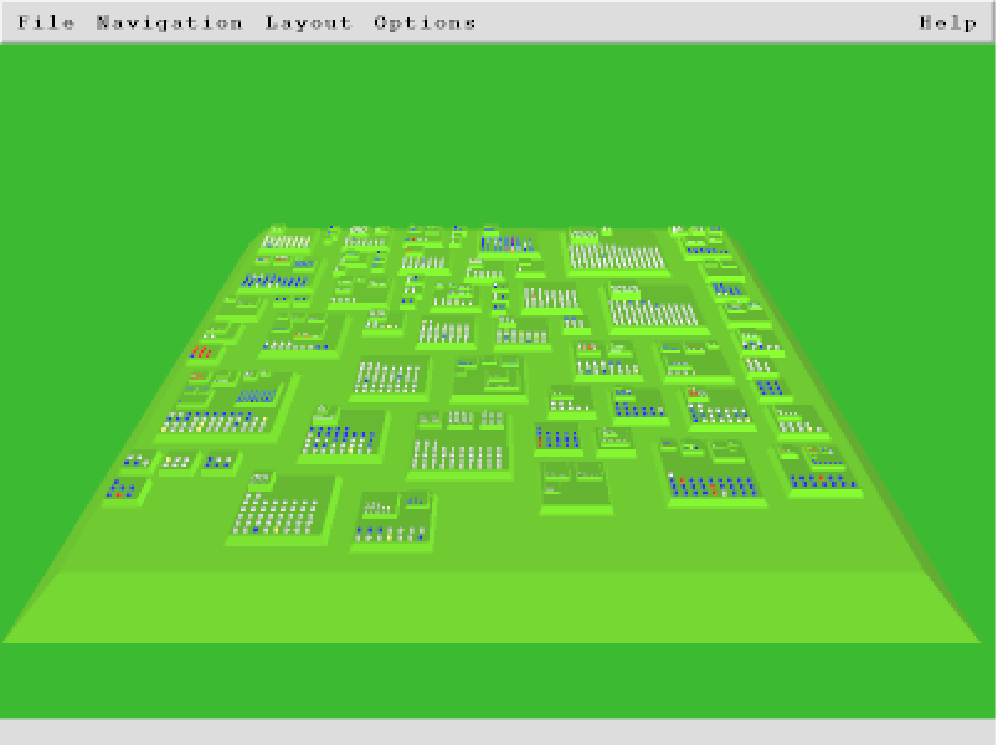
\includegraphics[width=\linewidth]{figures/information-pyramids}
		\caption{Übersicht} \label{fig:information-pyramids-overview}
	\end{subfigure}
	\hfill
	\begin{subfigure}{\fwidth}
		\centering
		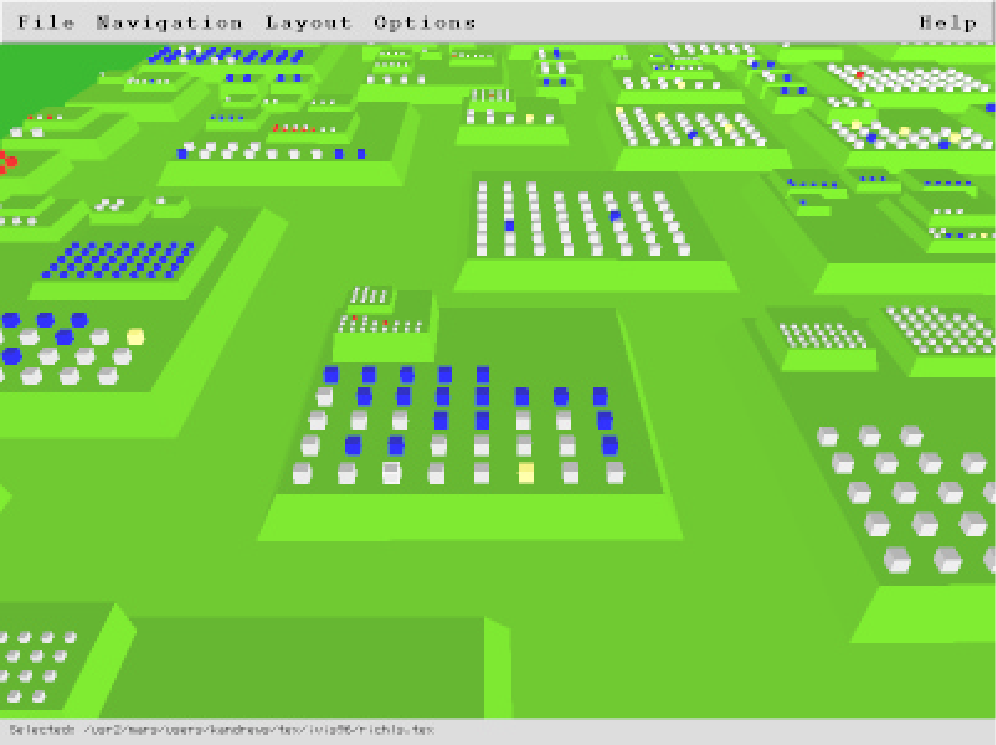
\includegraphics[width=\linewidth]{figures/information-pyramids-drilled}
		\caption{Detail-Ansicht} \label{fig:information-pyramids-drilled}
	\end{subfigure}
	\caption{Information Pyramids \cite{andrews1997information}} \label{fig:information-pyramids}
\end{figure}

\subsection{CodeCity von Wettel und Lanza}
\label{subsec:code-city}
 2007 stellten Wettel und Lanza ein Konzept vor, mit dem sich eine objektorientierte Software mithilfe der \textit{Stadt-Metapher} visualisieren ließ. Im Vordergrund dieser Herangehensweise der Visualisierung stand die Habitability, welche durch die Metapher und die damit einhergehende Möglichkeit der Orientierung erreicht werden sollte \cite{wettel2007Program}.
 
So wie bei Andrews et al. werden bei Wettel und Lanza Ordner bzw. Pakete durch Plateaus dargestellt, die jedoch weniger in die Höhe gehen sondern sich als Stadtviertel (engl. \textit{districts}) in die Stadt-Metapher einfügen.

In diesen Vierteln, die bei geschachtelten Paketen auch aufeinander geschichtet sein können, ragen dann Klassen als Gebäude in die Höhe.

Die Software kann dann laut Wettel und Lanza wie eine echte Stadt erkundet werden. Die Stadt im Ganzen vermittelt eine gute Übersicht über die Software und deren Komplexität. Einzelne Pakete können dann wie bei einem Stadtrundgang besichtigt und Klassen wie Häuser besucht werden.

Die Inhalte der Klassen werden nicht weiter visualisiert, da sie für das größer gefasstes Verständnis einer Software nicht notwendig sei.

Für die Breite und Tiefe der Gebäude wurde für die CodeCity die Anzahl der Attribute (engl. \textit{number of attributes (NOA)}) und für die Höhe die Anzahl der Methoden (engl. \textit{number of methods (NOM}) der visualisierten Klasse gewählt. In späteren Weiterentwicklungen der CodeCity wurden auch andere Metriken wie beispielsweise Komplexität unterstützt.

Für das Anordnung der Stadtviertel und der sich darin befindlichen Klassen verwendeten Wettel und Lanza einen \textit{rectangle-packing} \cite{wettel2007Program} Algorithmus, durch den die Elemente rekursiv der Größe nach in rechteckigen Grundflächen angeordnet werden.

In Abbildung \ref{fig:code-city} ist die Software ArgoUML als CodeCity abgebildet.


\begin{figure}[htbp]
	\centering
	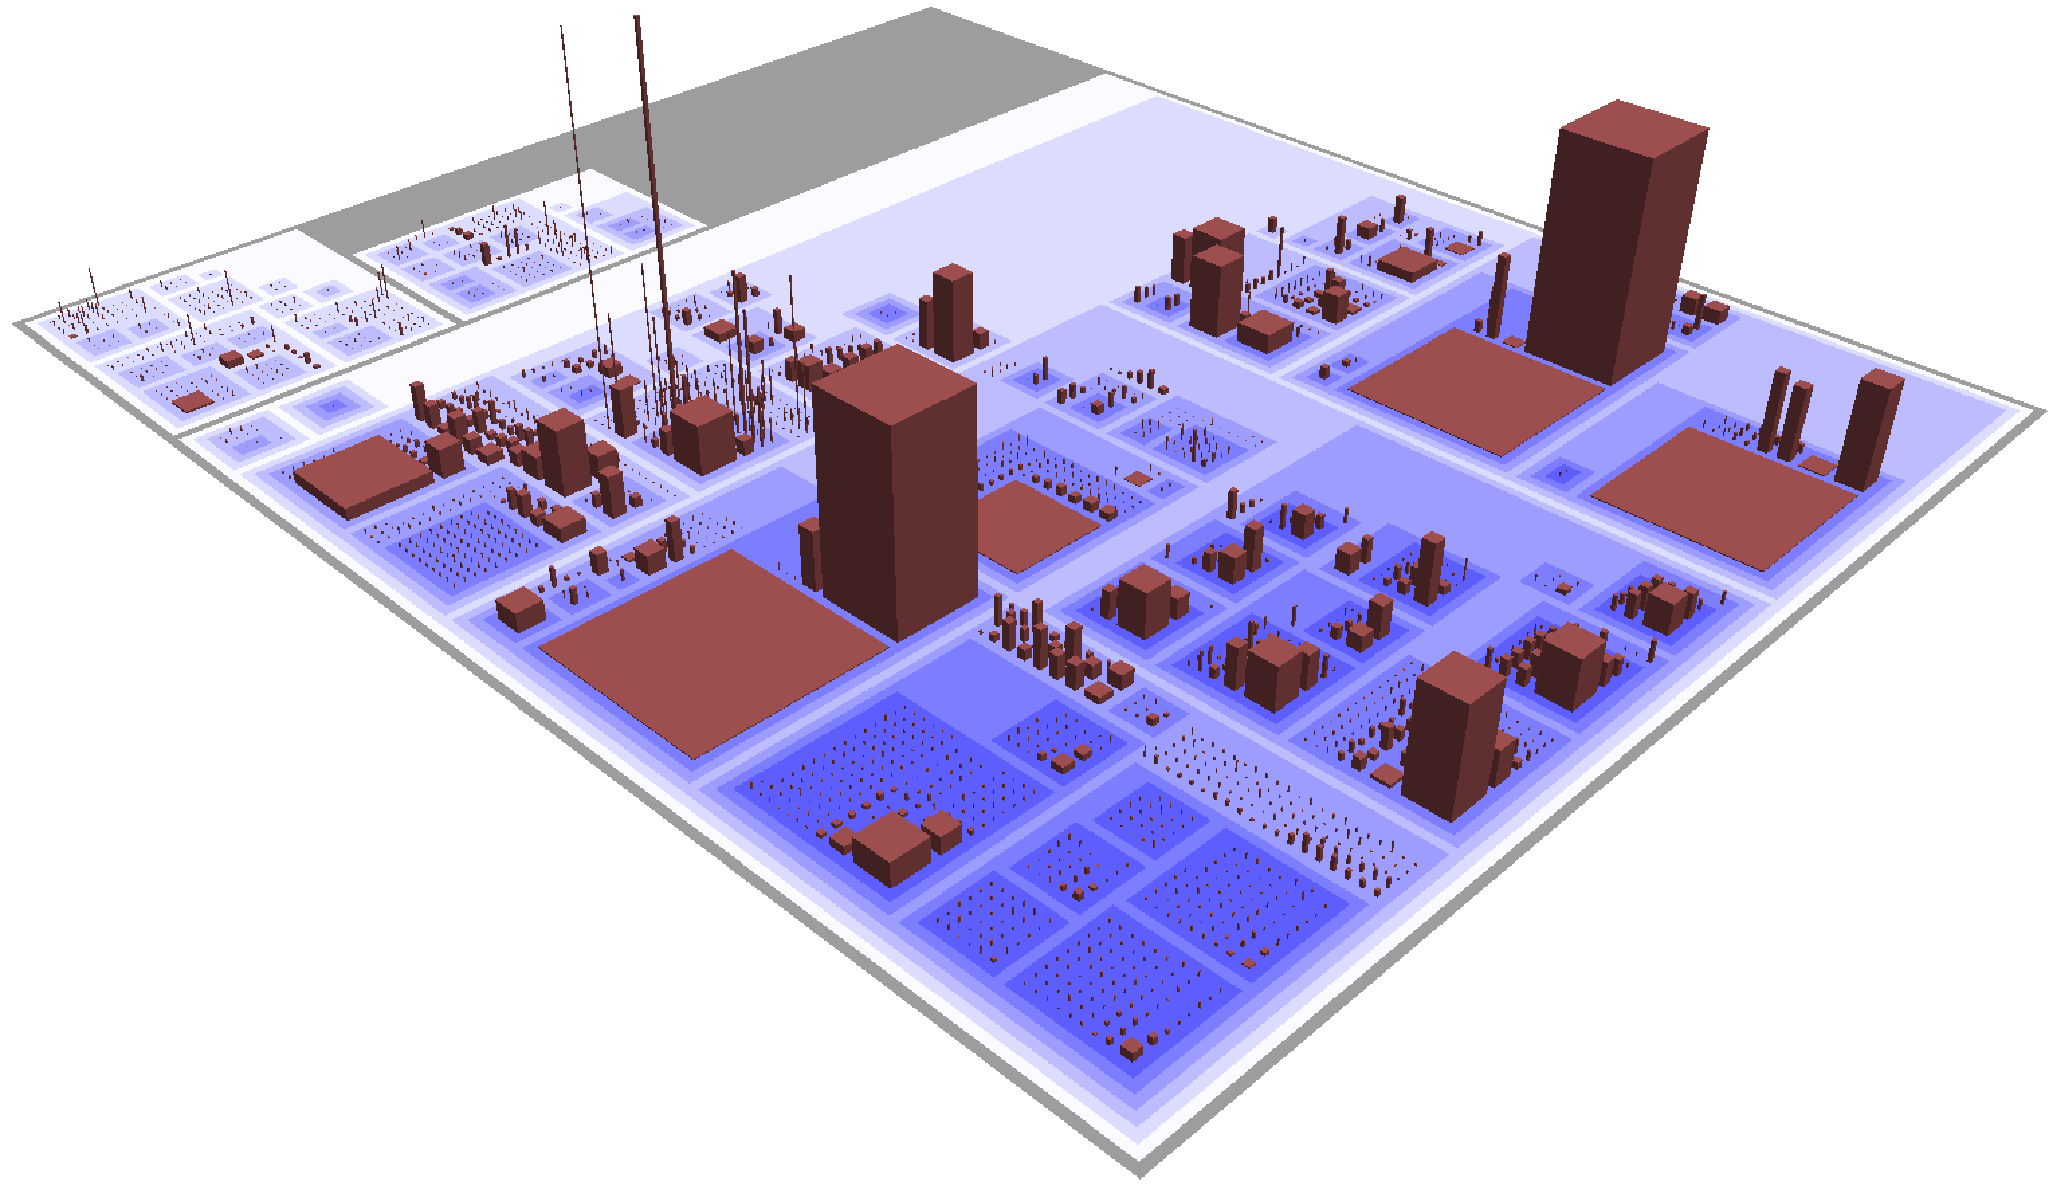
\includegraphics[width=\linewidth]{figures/code-city}
	\caption{CodeCity von ArgoUML \cite{wettel2008Visual}} \label{fig:code-city}
\end{figure}

Alternativ zu der linearen Darstellung der Größe der Gebäude, wurden auch Mapping Algorithmen untersucht, bei denen das Stadtbild harmonischer aussieht und die Habitability noch stärker angesprochen werden soll. Dabei werden die Klassen in Kategorien eingeteilt, die dann in sechs verschiedene Arten von Gebäuden -- von Haus (engl. \textit{house}) bis Wolkenkratzer (engl. \textit{skyscraper}) -- aufgeteilt werden.

\subsubsection*{Vorteile}
Die \textbf{Habitability} nimmt in der CodeCity einen großen Stellenwert ein, da das Modell primär dafür entworfen wurde.

Neben NOA und NOM ist in einer CodeCity auch S1 darstellbar. Die \textbf{Struktur} wird durch eine CodeCity sehr gut visualisiert und sogar \textbf{Abhängigkeiten} sind verfügbar. Die Abhängigkeiten von einer einzelnen Klasse ist in Abbildung \ref{fig:code-city-access} zu sehen.

Auch die \textbf{Evolution} einer Software kann durch ein Farbverlauf (in Abbildung \ref{fig:code-city-evolution} zu sehen) der Gebäude oder durch eine "`Zeitreise"' analysiert werden.

Der \textit{Drilldown} wird insofern unterstützt, dass einzelne UnterPakete in einem neuen Fenster geöffnet werden.

\setlength{\fwidth}{.49\textwidth}
\begin{figure}[htbp]
	\centering
	\begin{subfigure}[b]{0.9\fwidth}
		\centering
		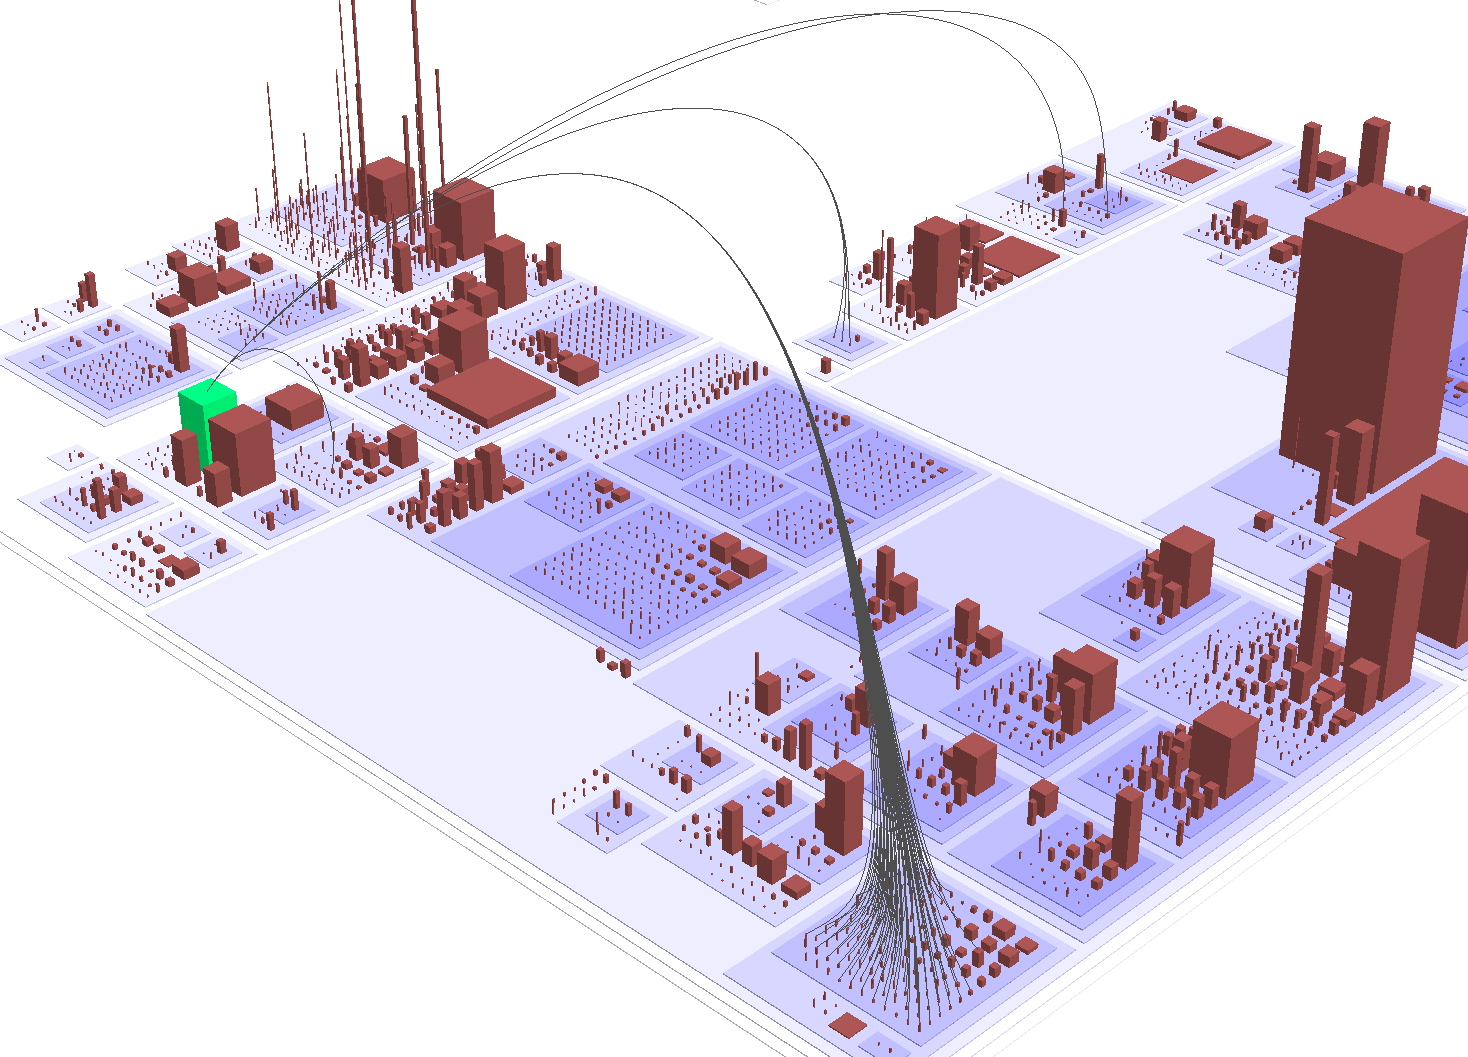
\includegraphics[width=\linewidth]{figures/code-city-access}
		\caption{Abhängigkeiten} \label{fig:code-city-access}
	\end{subfigure}
	\hfill
	\begin{subfigure}[b]{\fwidth}
		\centering
		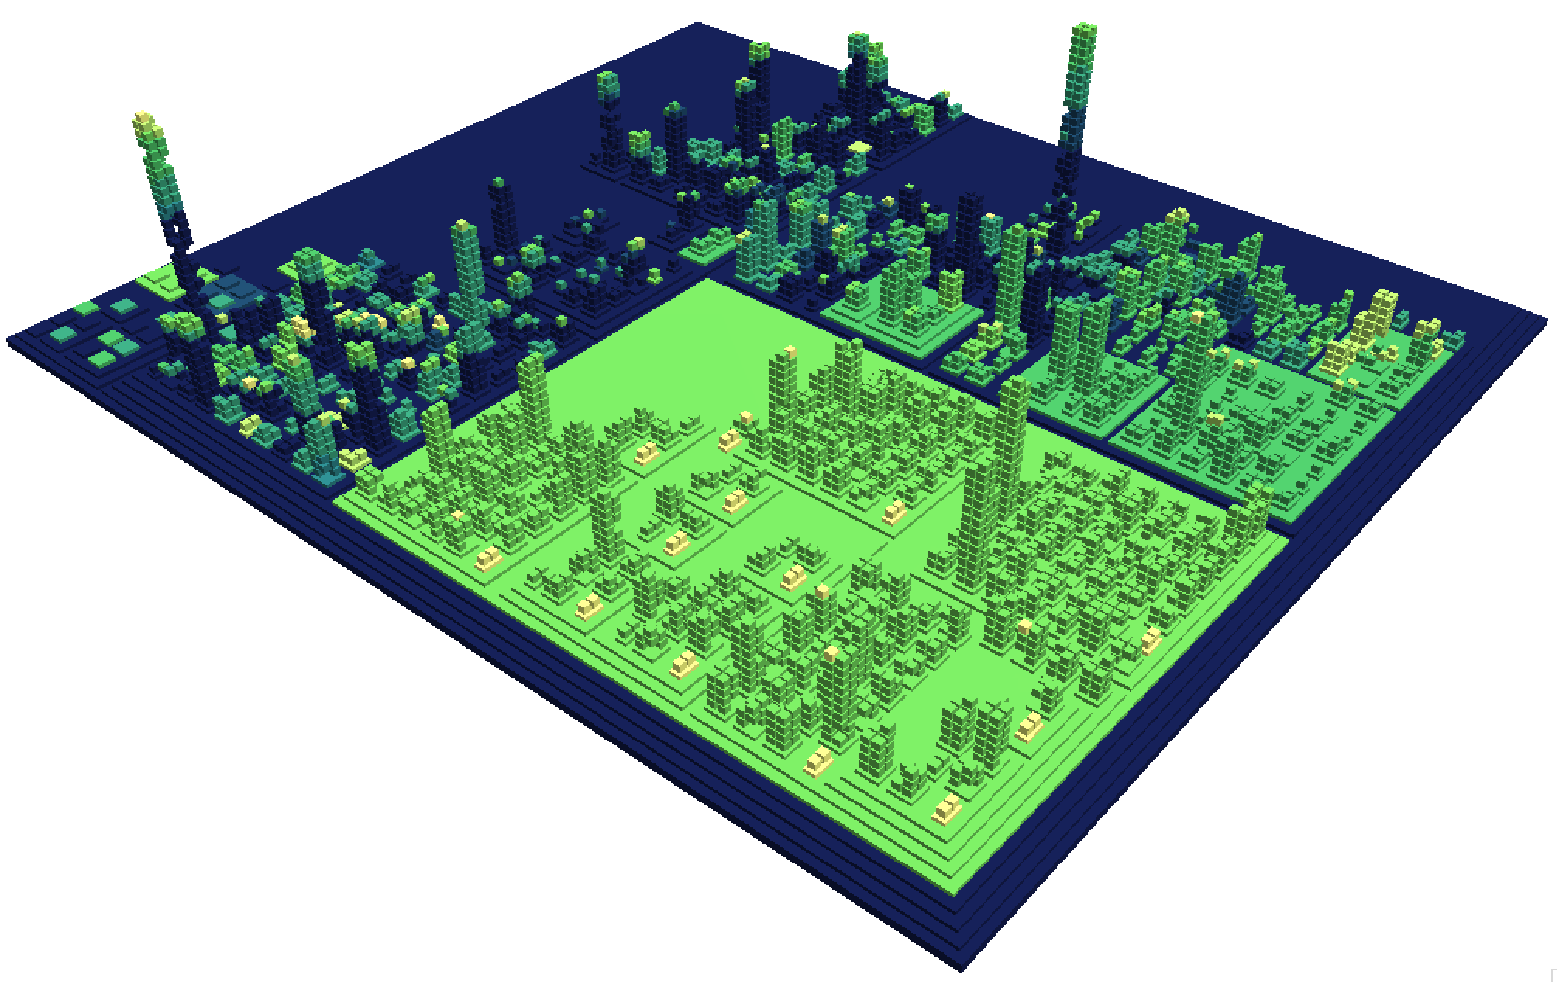
\includegraphics[width=\linewidth]{figures/code-city-evolution}
		\caption{Evolution \cite{wettel2008Visual}} \label{fig:code-city-evolution}
	\end{subfigure}
	\caption{Vorteile einer CodeCity} \label{fig:code-city-advantages}
\end{figure}

\subsubsection*{Nachteile}
Bei Betrachtung von Abhängigkeiten in ganzen Paketen oder des gesamten Systems werden die Abhängigkeiten schnell unübersichtlich. Die Abhängigkeiten sind alle einfarbig und werden können auch nur von dem aktuell ausgewählten Element angezeigt werden.

Der größte Nachteil der Implementierung der CodeCity ist die veraltete \textbf{Technologie}. Es wurde auf \textit{Moose}\footnote{\url{http://moosetechnology.org/}} gesetzt, eine Platform für die Analyse von Software \cite{merrill1916moose}. Moose wurde seit 1996 mit \textit{VisualWorks}\footnote{\url{http://www.cincomsmalltalk.com/main/products/visualworks/}} entwickelt, eine kommerzielle cross-platform Implementierung der Programmiersprache \textit{Smalltalk}. Smalltalk wurde in den frühen 1970ern im \textit{Xerox Palo Alto Research Center} entwickelt und ist eine der ersten objektorientierten Programmiersprache mit Konzepten, die zum Beispiel die JVM stark beeinflusst haben \cite{goldberg1983smalltalk}.

Seit 2008 wurde Moose von VisualWorks auf \textit{Pharao}\footnote{\url{http://pharo.org/}}, einer open-source Implementierung von Smalltalk, migriert. Seit 2009 wurde CodeCity nicht weiterentwickelt und auch der Workflow des Imports des Source-Code der zu visualisierende Software in ein von CodeCity lesbares Format, funktioniert heute nicht mehr so, wie es Wettel und Lanza dokumentiert hatten. Durch die Verwendung von Moose ist die 3D-Visualisierung der CodeCity auch für die Microsoft HoloLens nicht effektiv portierbar.

CodeCity weißt viele durchdachte Konzepte auf, ist jedoch 2017 nicht mehr für neue Software produktiv einsetzbar.

\subsection{SoftVis3D -- ein Plugin für SonarQube}

Eine ähnliche Implementierung der Stadt- Metapher wird seit 2012 von Rinderle entwickelt. Sein Projekt \textit{SoftVis3D}, das er im Rahmen seiner Master-Thesis ins Leben rief, ist ein Plugin für \textit{SonarQube}\footnote{\url{https://www.sonarqube.org/}}. SonarQube ist eine open-source Plattform für statische Code-Qualität. Die in Java entwickelte Software kann verschiedene Qualitätskriterien einer Momentaufnahme des betrachteten Source-Codes im Browser darstellen und ermöglicht darüber hinaus Trends zu erkennen \cite{campbell2013sonarqube}. Mithilfe von Plugins kann die Funktionalität bei der Aggregation der dargestellten Daten erweitert werden. Von neuen Metriken bis hin zu ganzen Programmiersprachen kann Funktionalität ergänzt werden.

Nicht nur für die Quelle der dargestellten Daten können Plugins entwickelt werden. Auch für Darstellung der aggregierten Daten ist es möglich eigene Plugins zu realisieren. SoftVis3D ist ein solches Plugin, das jegliches Projekt, das in SonarQube eingebunden ist, als Software-Stadt darstellen kann.

Das Grundprinzip von SoftViz3D ist das der CodeCity: Klassen werden als Häuser visualisiert. Die Konfigurierbarkeit ist jedoch bei SoftVis3D weitaus höher. Der Grundfläche und der Höhe der Häuser kann jegliche verfügbare Metrik von SonarQube zugeordnet werden. Für Java-Projekt ohne weitere Plugins sind dies 80 verschiedene Metriken. Für das Farbschema stehen sechs verschiedene Metriken, wie Complexity und Coverage zur Verfügung. Hervorzuheben ist die Metrik \textit{Package Name}, die Pakete und Klassen mit ähnlichem Namen in ähnlicher Farbe darstellt und so bei sprechender Benennung der Artefakte thematische Zusammengehörigkeit visualisiert.

Ein Java-Projekt der QAware mit 3.101 Klassen und 154,449 LOC als SoftVis3D Visualisierung ist in Abbildung \ref{fig:softvis3d} zu sehen. Als Konfiguration wurde Komplexität als Grundfläche, LOC als Höhe und Coverage als Farbe gewählt.

\begin{figure}[htbp]
	\centering
	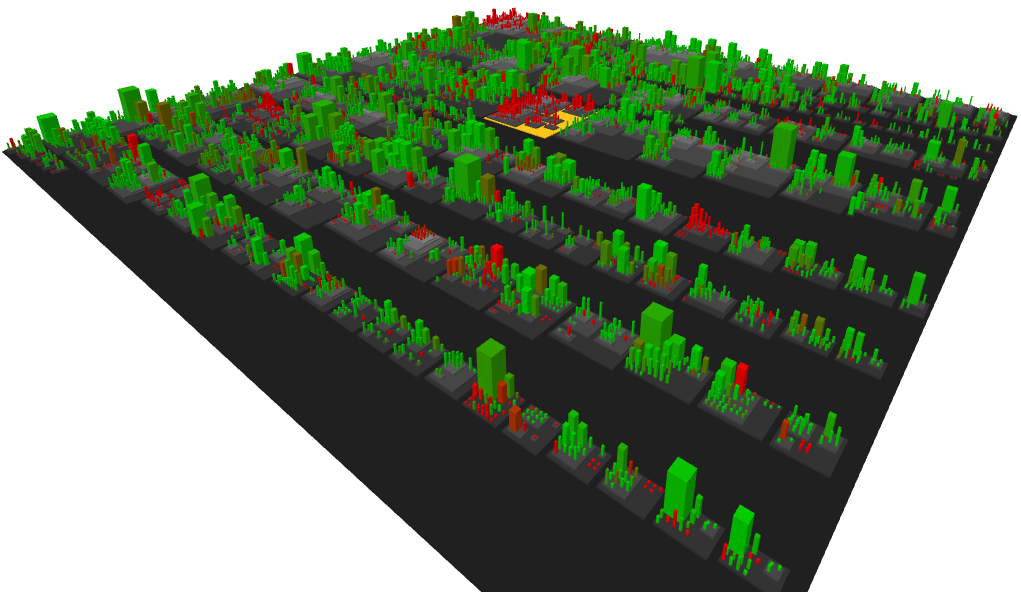
\includegraphics[width=\linewidth]{figures/softvis3d}
	\caption{SoftVis3D} \label{fig:softvis3d}
\end{figure}

Neben dem District-Layout, wie es auch in CodeCity Verwendung findet, wurde im Zuge der Master-Thesis von Niedrich eine zweite Layout Strategie für SoftVis3D realisiert \cite{niedrich2016integration}. Der sogenannte \textit{Evostreet}-Algorithmus wurde ursprünglich von Steinbrück für die besser Darstellung der Evolution einer Software entwickelt \cite{steinbruckner2013consistent}. Mit diesem Algorithmus soll sich die Struktur der Stadt nicht verändern und so eine Evolution der Software auch über längere Zeiträume ermöglichen. Die Pakete der Software werden nicht wie bei dem District-Layout als Plateaus dargestellt, sondern als Straßen. Das bedeutet das \textit{root}-Verzeichnis wird als Hauptstraße abgebildet und alle Unterpakete zweigen von dieser Straße ab. Alle weiteren UnterPakete verzweigen sich rekursiv weiter und einzelne Klassen werden am Ende einer Straße positioniert. Neue Klassen werden dadurch weitgehend am Rand der Stadt platziert, wodurch sich die Stadt mit der fortschreitender Zeit der Entwicklung nach außen hin ausbreitet.

Die Interaktion in SoftVis3D ist intuitiv gestaltet. Mit der Maus kann stufenlos in die Stadt hinein gezoomt und die Perspektive verändert werden. In Abbildung \ref{fig:softvis3d-layouts} kann eine Detailansicht vom District-Layout und vom Evostreet-Layout betrachtet werden.

\setlength{\fwidth}{.49\textwidth}
\begin{figure}[htbp]
	\centering
	\begin{subfigure}[b]{\fwidth}
		\centering
		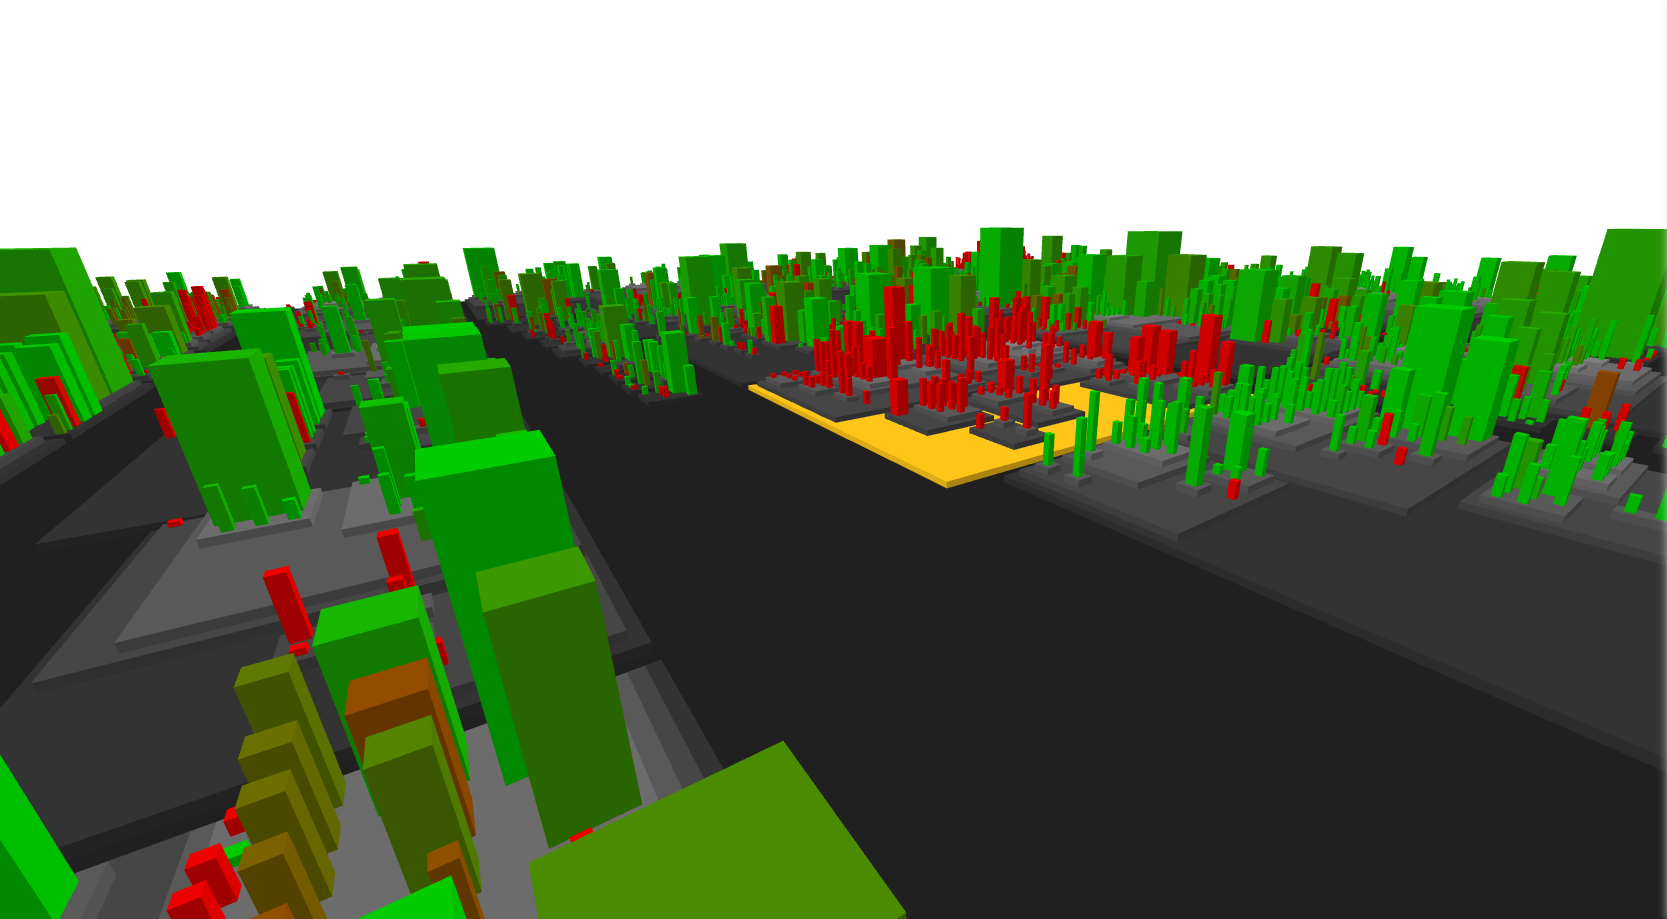
\includegraphics[width=\linewidth]{figures/softvis3d-district}
		\caption{District Layout} \label{fig:softvis3d-district}
	\end{subfigure}
	\hfill
	\begin{subfigure}[b]{\fwidth}
		\centering
		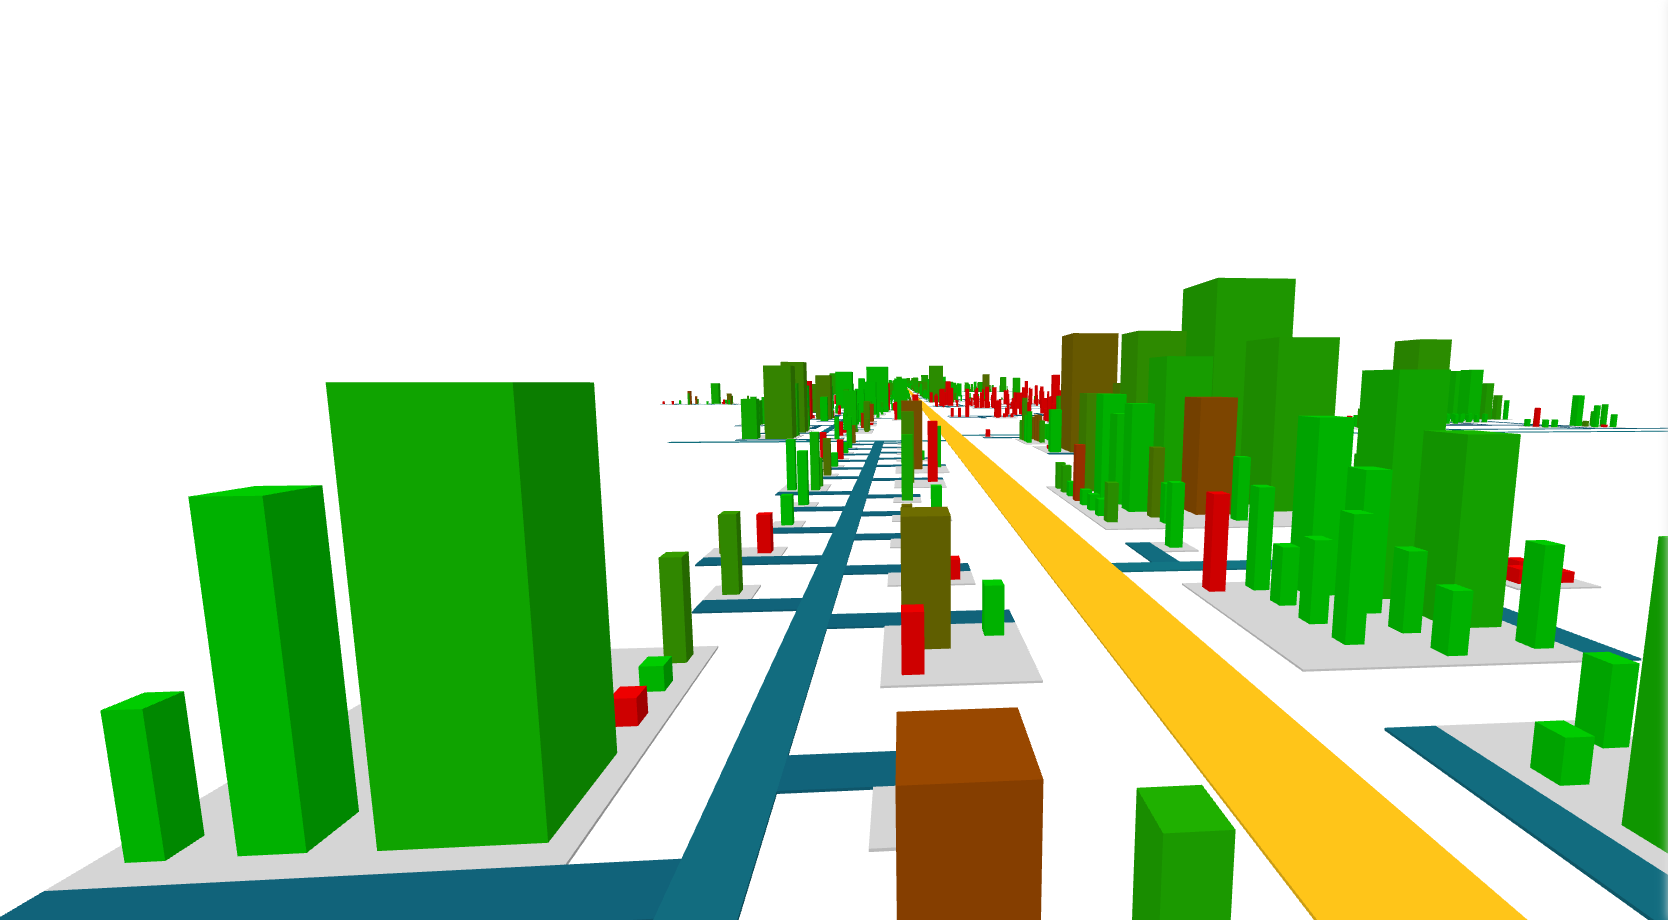
\includegraphics[width=\linewidth]{figures/softvis3d-evostreet}
		\caption{Evostreet Layout} \label{fig:softvis3d-evostreet}
	\end{subfigure}
	\caption{Unterstützte Layouts von SoftVis3D} \label{fig:softvis3d-layouts}
\end{figure}

Alle Artefakte der Stadt können ausgewählt werden (in Abbildung \ref{fig:softvis3d} und \ref{fig:softvis3d-layouts} gelb markiert), woraufhin in einem Menu alle Kinder gelistet werden können. Zusätzlich kann aus dem Plugin heraus direkt in den Source-Code einer ausgewählten Klasse gesprungen werden.

Ein weiterer Unterschied zur CodeCity ist die Darstellung der Abhängigkeiten in SoftVis3D. Die aktuellen Version des SonarQube Plugins unterstützt die Darstellung der Abhängigkeiten zwar nicht, jedoch hat Rinderle 2016 in \cite{rinderle2016kontinuierliche} dazu ein Konzept vorgestellt indem die Abhängigkeiten einer Software in einer Software-Stadt mit mehreren Ebenen visualisiert werden. Dazu werden die Abhängigkeiten aggregiert. Aggregation von Abhängigkeiten lässt sich allgemein folgendermaßen definieren:

\newtheorem{aggregation}{Definition}[section]
\begin{aggregation}\label{def:aggregation}
Bei der Aggregation von Abhängigkeiten zwischen Klassen werden die Abhängigkeiten nicht als direkte Verbindungen dargestellt, sondern über die Eltern-Pakete geleitet. Eine Klasse $A \in x$ (im Paket $x$) besitzt eine Abhängigkeit zu Klasse $B \in y$. Die Abhängigkeit von $A$ geht zu einem zusätzlich Konstrukt $\Psi_x$, das die Außensicht des Pakets $x$ repräsentiert. Angenommen $x$ und $y$ befinden sich im Paket $z$, dann geht die aggregierte Abhängigkeit entweder direkt von $\Psi_x$ zu $\Psi_y$, oder geht über $\Psi_z$ zu $\Psi_y$ und die Hierarchie weiter nach unten zu $B_y$.
\end{aggregation}

In SoftVis3D werden Abhängigkeiten zwischen Klassen innerhalb eines Pakets werden nicht aggregiert, sondern direkt als Pfeile angezeigt. Abhängigkeiten über Paketgrenzen hinweg werden aggregiert angezeigt und $\Psi$ wird als zusätzliches Gebäude realisiert, wie es in Abbildung \ref{fig:softvis3d-aggregation} zu sehen ist. Für jede Hierarchie-Ebene wird eine neue Ebene verwendet. Die zusätzlichen Gebäude enden in der jeweils darüber liegenden Ebene in einem Plateau, das die Größe des Pakets darunter widerspiegelt. Die aggregierten Abhängigkeiten werden dann zwischen den Plateaus dargestellt.

\begin{figure}[htbp]
	\centering
	\begin{subfigure}[b]{.3\textwidth}
		\centering
		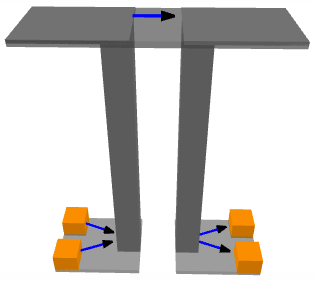
\includegraphics[width=\linewidth]{figures/softvis3d-aggregation}
		\caption{Aggregation von Abhängigkeiten in SoftVis3D} \label{fig:softvis3d-aggregation}
	\end{subfigure}
	\hfill
	\begin{subfigure}[b]{.6\textwidth}
		\centering
		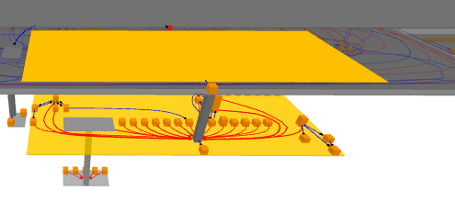
\includegraphics[width=\linewidth]{figures/softvis3d-dependencies}
		\caption{Ausschnitt aus dem Projekt Groovy} \label{fig:softvis3d-groovy}
	\end{subfigure}
	\caption{Abhängigkeiten in SoftVis3D \cite{rinderle2016kontinuierliche}} \label{fig:softvis3d-dependencies}
\end{figure}

\subsubsection*{Vorteile}

Bei der Visualisierung verschiedener \textbf{statischen Metriken von Klassen} kann SoftVis3D punkten. Die ganze Vielfalt an Metriken, die SonarQube unterstützt, kann auch in SoftVis3D Verwendung finden. SoftVis3D unterstützt für die \textbf{Struktur} der Software sogar verschiedene Layouts, wodurch das am besten für den jeweiligen Use-Case passende Layout gewählt werden kann. Wie auch bei der CodeCity ist die \textbf{Habitability} durch die Stadt-Metapher sehr gut und der \textbf{Drilldown} ist durch die intuitive Interaktion bei SoftVis3D noch besser.

\subsubsection*{Nachteile}

Die Darstellung der Abhängigkeiten beeinflusst die Darstellung der Struktur der Software, da zusätzliche Hilfsgebäude und mehrere Ebenen gebraucht werden. Die Übersichtlichkeit des 3D-Modells wird dadurch stark negativ beeinflusst.

Wie auch bei der CodeCity sind \textbf{Dynamische} Metriken nicht Teil des Modells.

Auch wenn mit dem Evostreet-Algorithmus ein Layout für eine Visualisierung der \textbf{Evolution} gegeben wäre, gibt es in SoftVis3D keine Möglichkeit diese auf einen Blick darzustellen.

Da SoftVis3D für den Browser konzipiert ist, wurde das Plugin \textbf{technologisch} auf \textit{WebGL}-Basis mit \textit{three.js}\footnote{JavaScript 3D Library \url{https://threejs.org/}} entwickelt. WebGL wird jedoch nicht nativ auf der Microsoft HoloLens unterstützt. Ergo ist eine Verwendung oder Erweiterung von SoftVis3D für die Verwendung auf der Microsoft HoloLens nicht ohne Weiteres möglich. Ob das Rendern des SoftVis3D-Modells überhaupt mit tragbarem Aufwand für die Microsoft HoloLens verwendbar ist, soll teil der technischen Machbarkeit in Kapitel \ref{sec:technologie} sein.

\section{Alternative Ansätze}\label{sec:alternatives}
Es wurden bisher zwei Umsetzungen der Stadt-Metapher behandelt. In diesem Abschnitt der Arbeit soll durch die kreative Entwicklung eigener Metaphern zwei Alternativen beleuchtet werden und ebenfalls anhand der in Abschnitt \ref{subsec:categories} aufgestellten Kriterien bewertet werden.

\subsection{CodeForest}

Die Softwarevisualisierung beschäftigt sich im Allgemeinen meist mit der Darstellung von hierarchischen Informationen. ``Hierarchies are almost ubiquitous [...]''\footnote{dt.: "`Hierarchien sind fast allgegenwärtig [...]"'} \cite{robertson1991cone}, stellten Robertson et al. schon 1991 bei der Visualisierung von hierarchischen Informationen fest.

Die Struktur einer Software mit geschachtelten Paketen entspricht immer der einer Baumstruktur. In der Informatik weit verbreitet, ist diese Struktur auch nichts Anderes als eine Metapher. Die Ursprung entstammt einer Realität, die sich jeder gut vorstellen kann -- eines Baumes. Zwar wird die Baumstruktur in der Informatik schon seit jeher zweidimensional verwendet, jedoch wäre eine dreidimensionale Visualisierung, der eigentlichen Metapher folgend, nur logisch. Wieso also nicht Software als dreidimensionale Bäume visualisieren?

Diesem Ansatz nachgehend, entsteht das Modell des \textit{CodeForest}. Die Bäume werden in "`Wuchsrichtung"' auf einer Ebene dargestellt. Die Analogie in diesem Modell ist simpel. Einzelne Bäume stellen Pakete im root-Verzeichnis der Software da, Verzweigungen Unterpakete und die Blätter der Bäume stellen die eigentlichen Dateien der Software dar. Die darzustellenden Metriken können dann als "`Laubfärbung"' angewandt werden. 

Es können einzelne Pakete genauer betrachtet werden, indem ein spezielles Paket das neue root-Verzeichnis wird und alle Unterpakete als neue Bäume auf der Ebene stehen.

Die Evolution einer Software ist durch das Wachstum des Waldes möglich zu visualisieren.

Besonders interessant ist die Visualisierung der Abhängigkeiten. In zwei Dimensionen sind Verbindungen zwischen Wurzel-Elementen nicht oder bestenfalls schlecht darstellbar. In drei Dimensionen gewinnt die Metapher von Bäumen an einem neuen Element -- dem "`Wurzelgeflecht"'. Was im Zweidimensionalen hinter einer einzelnen Verbindung zwischen den Wurzel-Elementen verschwinden würde, spannt sich nun mit dem Wurzelgeflecht auf dem Waldboden auf.

Ähnlich wie bei dem Ansatz der Abhängigkeiten in SoftVis3D können Abhängigkeiten zwischen Paketen aggregiert werden und dann zwischen den Bäumen als Wurzeln visualisiert werden. Ungewünschte Abhängigkeiten, wie zum Beispiel zyklische, können direkt in den Bäumen farbig in der entsprechenden "`Verästelung"' hervorgehoben werden.

\begin{figure}[htbp]
	\centering
	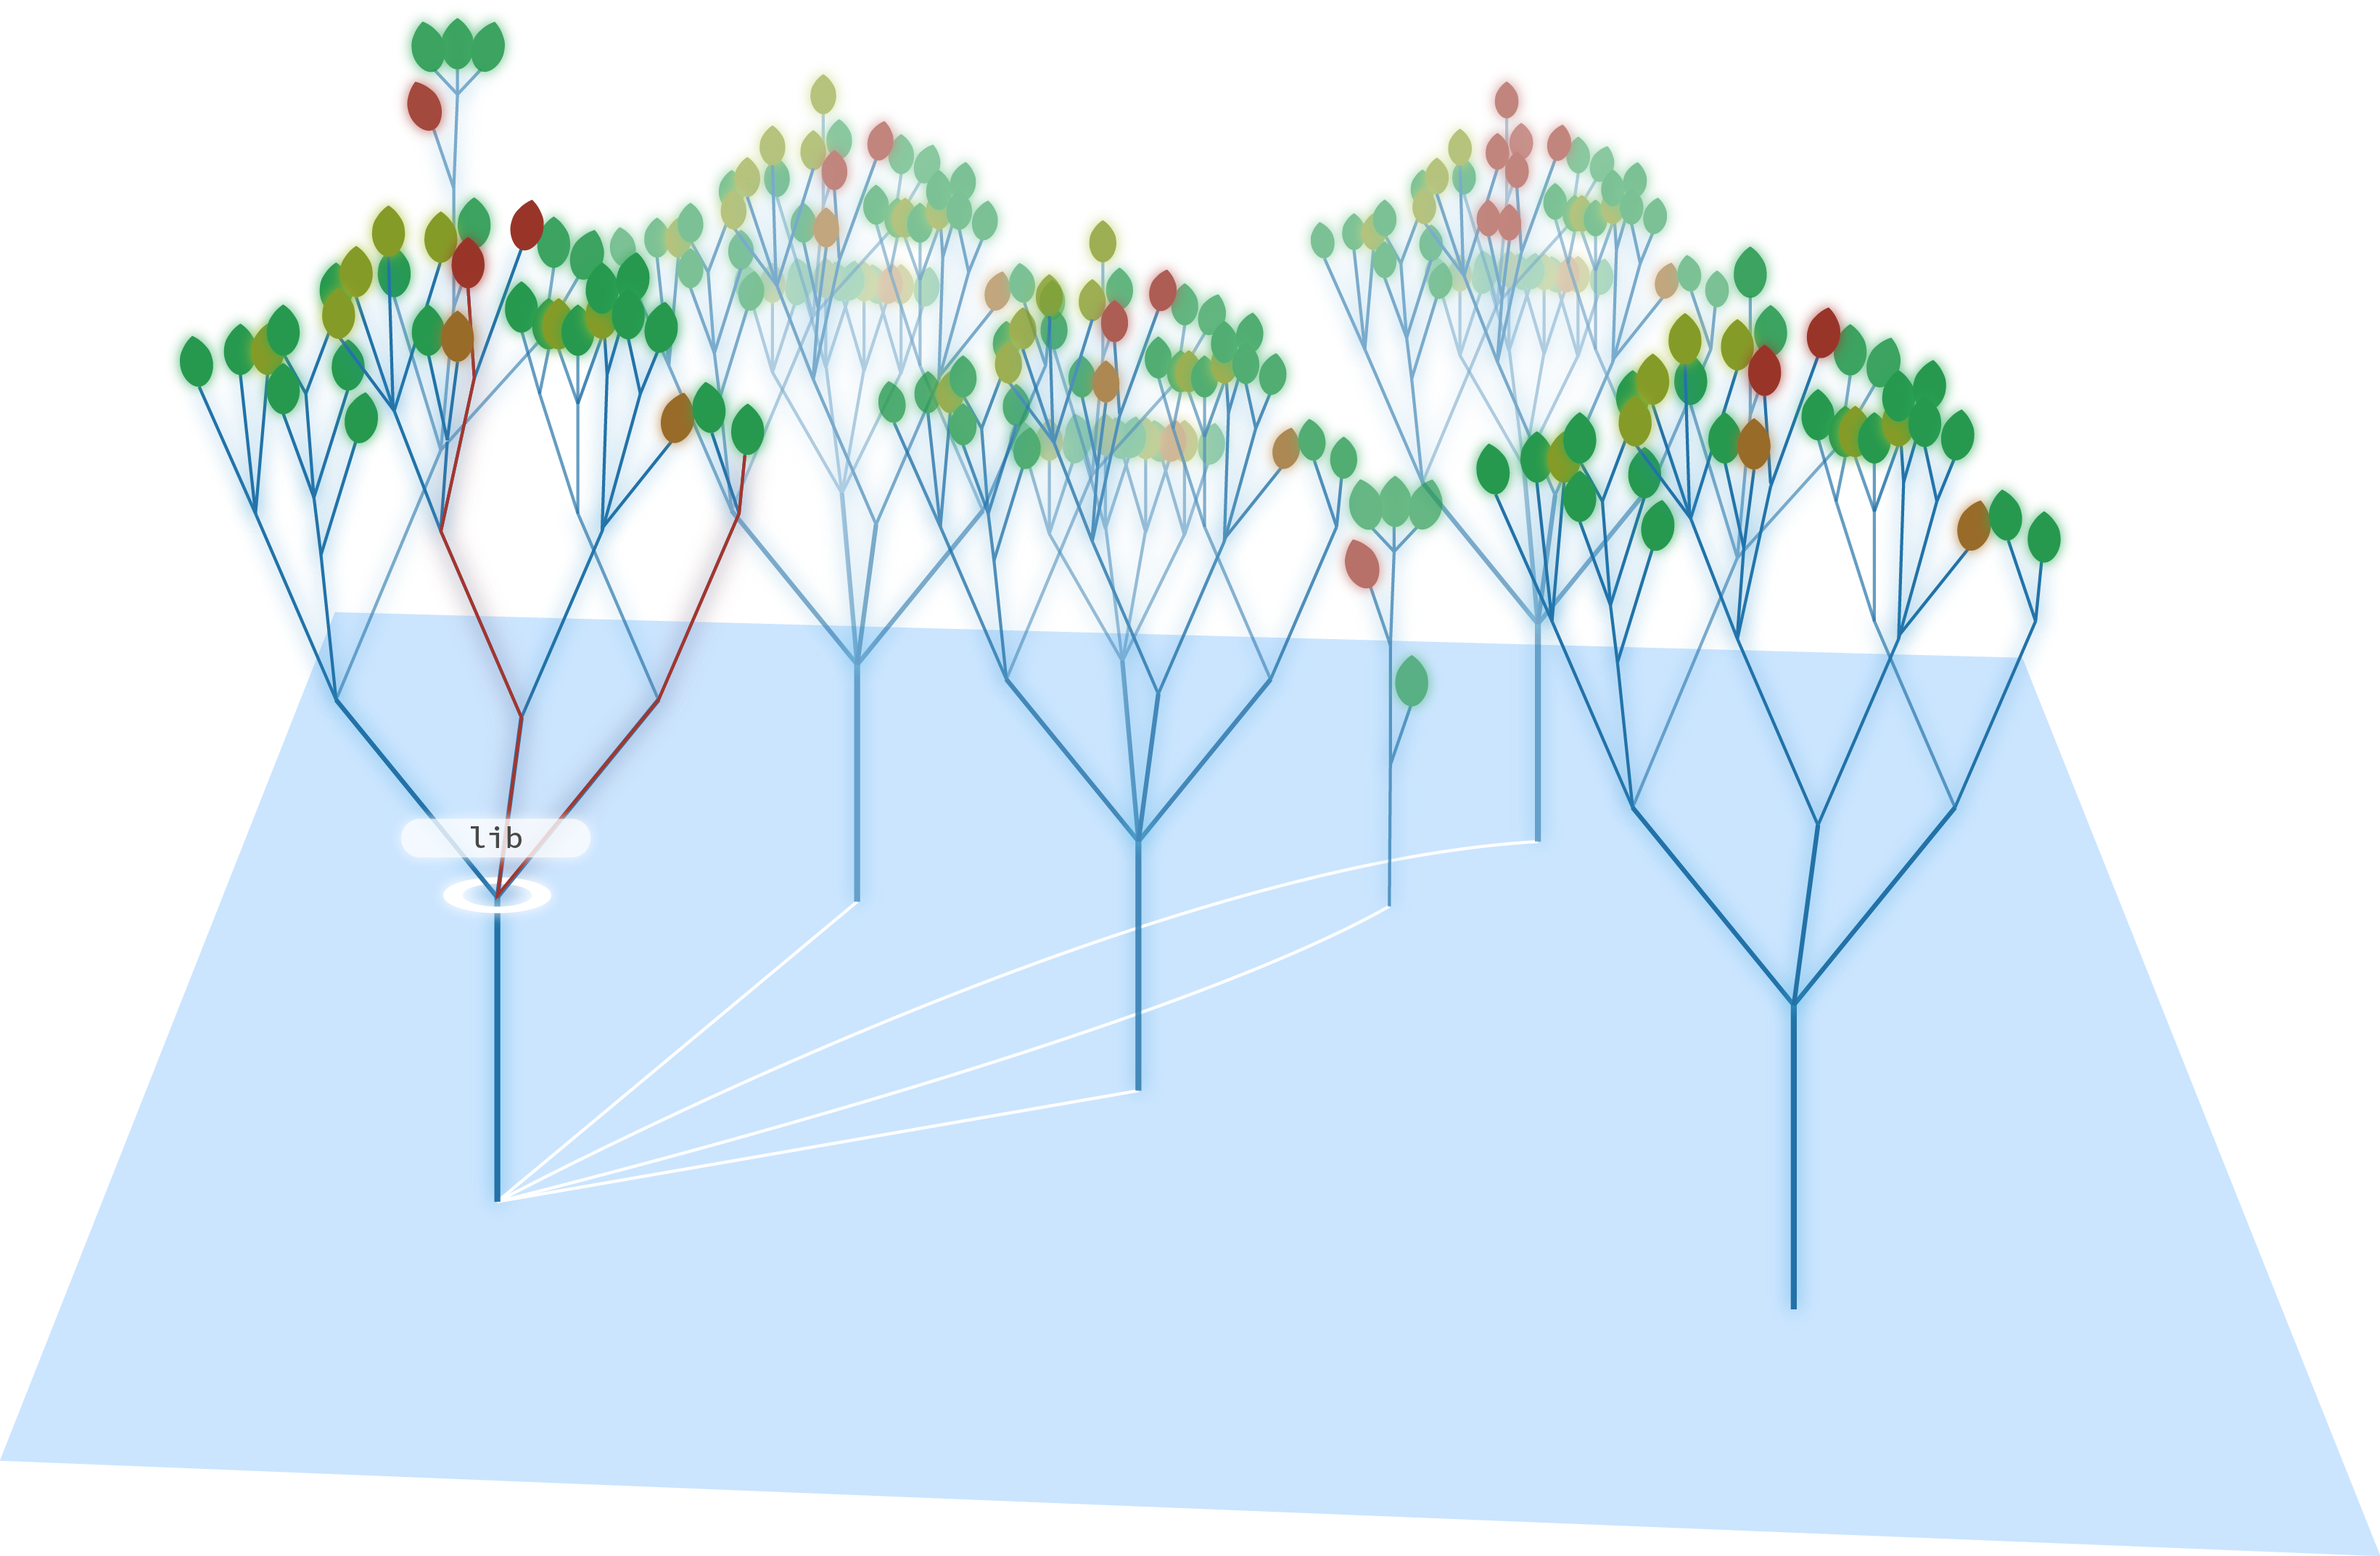
\includegraphics[width=\linewidth]{figures/code-forest}
	\caption{Beispielhafter Entwurf eines CodeForest} \label{fig:code-forest}
\end{figure}

Zu dieser reduzierbaren, aber übersichtlichen Darstellung der Abhängigkeiten sind noch zwei weitere Darstellungsformen denkbar. Zum einen können alle Abhängigkeiten von einem ausgewählten Blatt den Stamm hinunter über die Wurzeln, den Astverlauf hinauf bis hin zum Ziel-Blatt dargestellt werden, wodurch eine genauere Untersuchung der Abhängigkeiten möglich ist. Zum andern wäre für eine Gesamtdarstellung auch eine direkte Verbindung der Blätter durch "`Spinnweben"' zwischen den Bäumen denkbar.

In Abbildung \ref{fig:code-forest} ist beispielhaft ein solcher CodeForest illustriert. Es ist das Paket \texttt{lib} im root-Verzeichnis ausgewählt. Es werden die aggregierten Abhängigkeiten zu anderen Bäumen dargestellt und eine ungewünschte Abhängigkeit innerhalb des ausgewählten Pakets existiert.

\subsubsection*{Nachteile}
Gegenüber der Stadt-Metapher hat die Wald-Metapher den Nachteil, dass lediglich mit der Farbe der Blätter und damit nur eine \textbf{statische Metrik} gleichzeitig darstellbar ist. Bei der Stadt-Metapher sind es mit Grundfläche, Höhe und Farbe der Gebäude 3 Metriken gleichzeitig.

\subsubsection*{Vorteile}
Die \textbf{Struktur} der Software wird durch Eins-zu-eins-Um­set­zung auf die Bäume sehr gut widergespiegelt. \textbf{Abhängigkeiten} können durch das Wurzelgeflecht auf verschiedener Schachtelungstiefe, farbige Verästelung oder alternativen Spinnweben sehr interaktiv dargestellt werden.

Die \textbf{Evolution} der betrachteten Software integriert sich mit dem Wachstum eines Waldes nahtlos in die Wald-Metapher.

Die Darstellung der \textbf{Dynamik} bzw. Aufrufe können mithilfe von Verbindung, wie sie bei den Abhängigkeiten zum Einsatz kommen, dargestellt werden. Zudem könnte die Stamm- bzw. Ast-Dicke ein Indikator für die Anzahl der Aufrufe sein. Die Laufzeiten kann sich in der Farbe des Laubwerks wieder spiegeln.

Durch die Struktur der Bäume ist die Habitability gut umgesetzt. Ein Entwickler, der mit der Code-Base vertraut ist, wird sich im CodeForest schnell zurecht finden können. Jedoch können Bäume weniger markant eingeschätzt werden, als Stadt-Vierteln mit markanten Gebäuden.

Der Drilldown ist durch die "`Verschiebung des Waldbodens nach oben"' interaktiv gestaltbar.

\subsection{CodeUniverse}

Bei der Suche nach einer weiteren eventuell geeigneten Metapher für die Darstellung von Software stellte sich die Frage, mit welchem Modell sich potentiell sehr viele Artefakte darstellen lassen können. Die Idee ein Universum als Softwarevisualisierung zu verwenden, lag dabei nicht fern. Im Folgendem wird deshalb das Modell \textit{CodeUniverse} vorgestellt.

Tatsächlich stellte sich nach einer Recherche heraus, dass sich in \cite{balzer2004software} aus 2004 von Balzer et al. ein ähnlicher Ansatz finden lässt. Hier wird zwar nicht von einem Universum gesprochen, aber von geschachtelten Sphären: ``The hierarchy of packages, which can be arbitrarily deep, is represented by nested spheres. The outermost sphere stands for the root of the package hierarchy.''\footnote{dt.: Die Hierarchie der Pakete, die beliebig tief sein kann, wird durch geschachtelte Sphären repräsentiert. Die äußerste Sphäre entspricht dem root-Verzeichnis der Paket-Hierarchie.} \cite{balzer2004software} Genau das ist das Grundprinzip. Bei Balzer et al. sind die Sphären von außen undurchsichtig. Erst beim Zoom in eine Sphäre wird die Hülle durchsichtig und offenbart weitere Sphären. Für einen Drilldown wäre das eine gute Alternative, für die Metapher des Universums und der Übersicht über eine Software, wäre es aber besser alle Artefakte der Software als sichtbare Sterne darzustellen. Die Sphären können aber dennoch für die Zugehörigkeit zu den Paketen um die Sterne als "`Nebel dargestellt werden"'.

Die Zugehörigkeit zu einem Paket wird aber auch über die Distanz der Sterne zueinander deutlich. Die Sterne des Pakets mit der tiefsten Hierarchie liegen am nächsten zusammen. Je näher am root-Verzeichnis, desto weiter dehnt sich das Universum aus, um innerhalb eines Pakets zwischen den Unterpaketen bzw. einzelnen Klassen gleich viel Abstand zu haben.

Die Größe und Farbe der Sterne -- von "`Weißen Zwergen"' bis hin zu "`Roten Riesen"' --lässt sich jeweils einer Metrik zuordnen. Beispielsweise stechen dann besonders große, in entsprechender Farbe leuchtende Sterne gut ins Auge.

Abhängigkeiten können als direkte Verbindungen dargestellt werden, oder wiederum aggregiert (vgl. Definition \ref{def:aggregation}) werden. Dabei würden Verbindungen zwischen den Sphären der einzelnen Pakete entstehen.

In Abbildung \ref{fig:code-universe} ist ein beispielhafter Entwurf eine kleinen CodeUniverse abgebildet. Es ist das root-Verzeichnis mit zwei einzelnen Klassen und vier Unterpaketen dargestellt. In diesem Beispiel wurde für Abhängigkeiten direkte Verbindung gewählt und eine unerwünschte Abhängigkeit farbig hervorgehoben.

\subsubsection*{Vorteile}
Im Vergleich zum CodeForest, kann das CodeUniverse gleichzeitig eine \textbf{statische Metrik} mehr anzeigen.

Die \textbf{Evolution} ist in einem CodeUniverse durchaus gut darstellbar. Das Wachstum der Software könnte als "`Ausdehnung"' des Universums visualisiert werden.

Im Vergleich zur CodeCity wären \textbf{Abhängigkeiten} als direkte Verbindungen übersichtlicher, da in einer CodeCity Verbindungen nur überhalb der Stadt sein können. Im CodeUnivers können Verbindungen in alle Richtungen gehen. Weiterhin sind Abhängigkeiten, die hierarchisch nur nach oben bzw. unten gehen, d.h. keine Nachbarpakete beinhalten, aufgrund des ausdehnenden Anordnung der Sterne mit wenig Überschneidungen darstellbar.

Der \textbf{Drilldown} ist mit "`Öffnen neuer Galaxien"' sehr gut und auch die \textbf{Habitability} ist mit der unterschiedlichen Ausdehnung der Galaxien gut.

\begin{figure}[htbp]
	\centering
	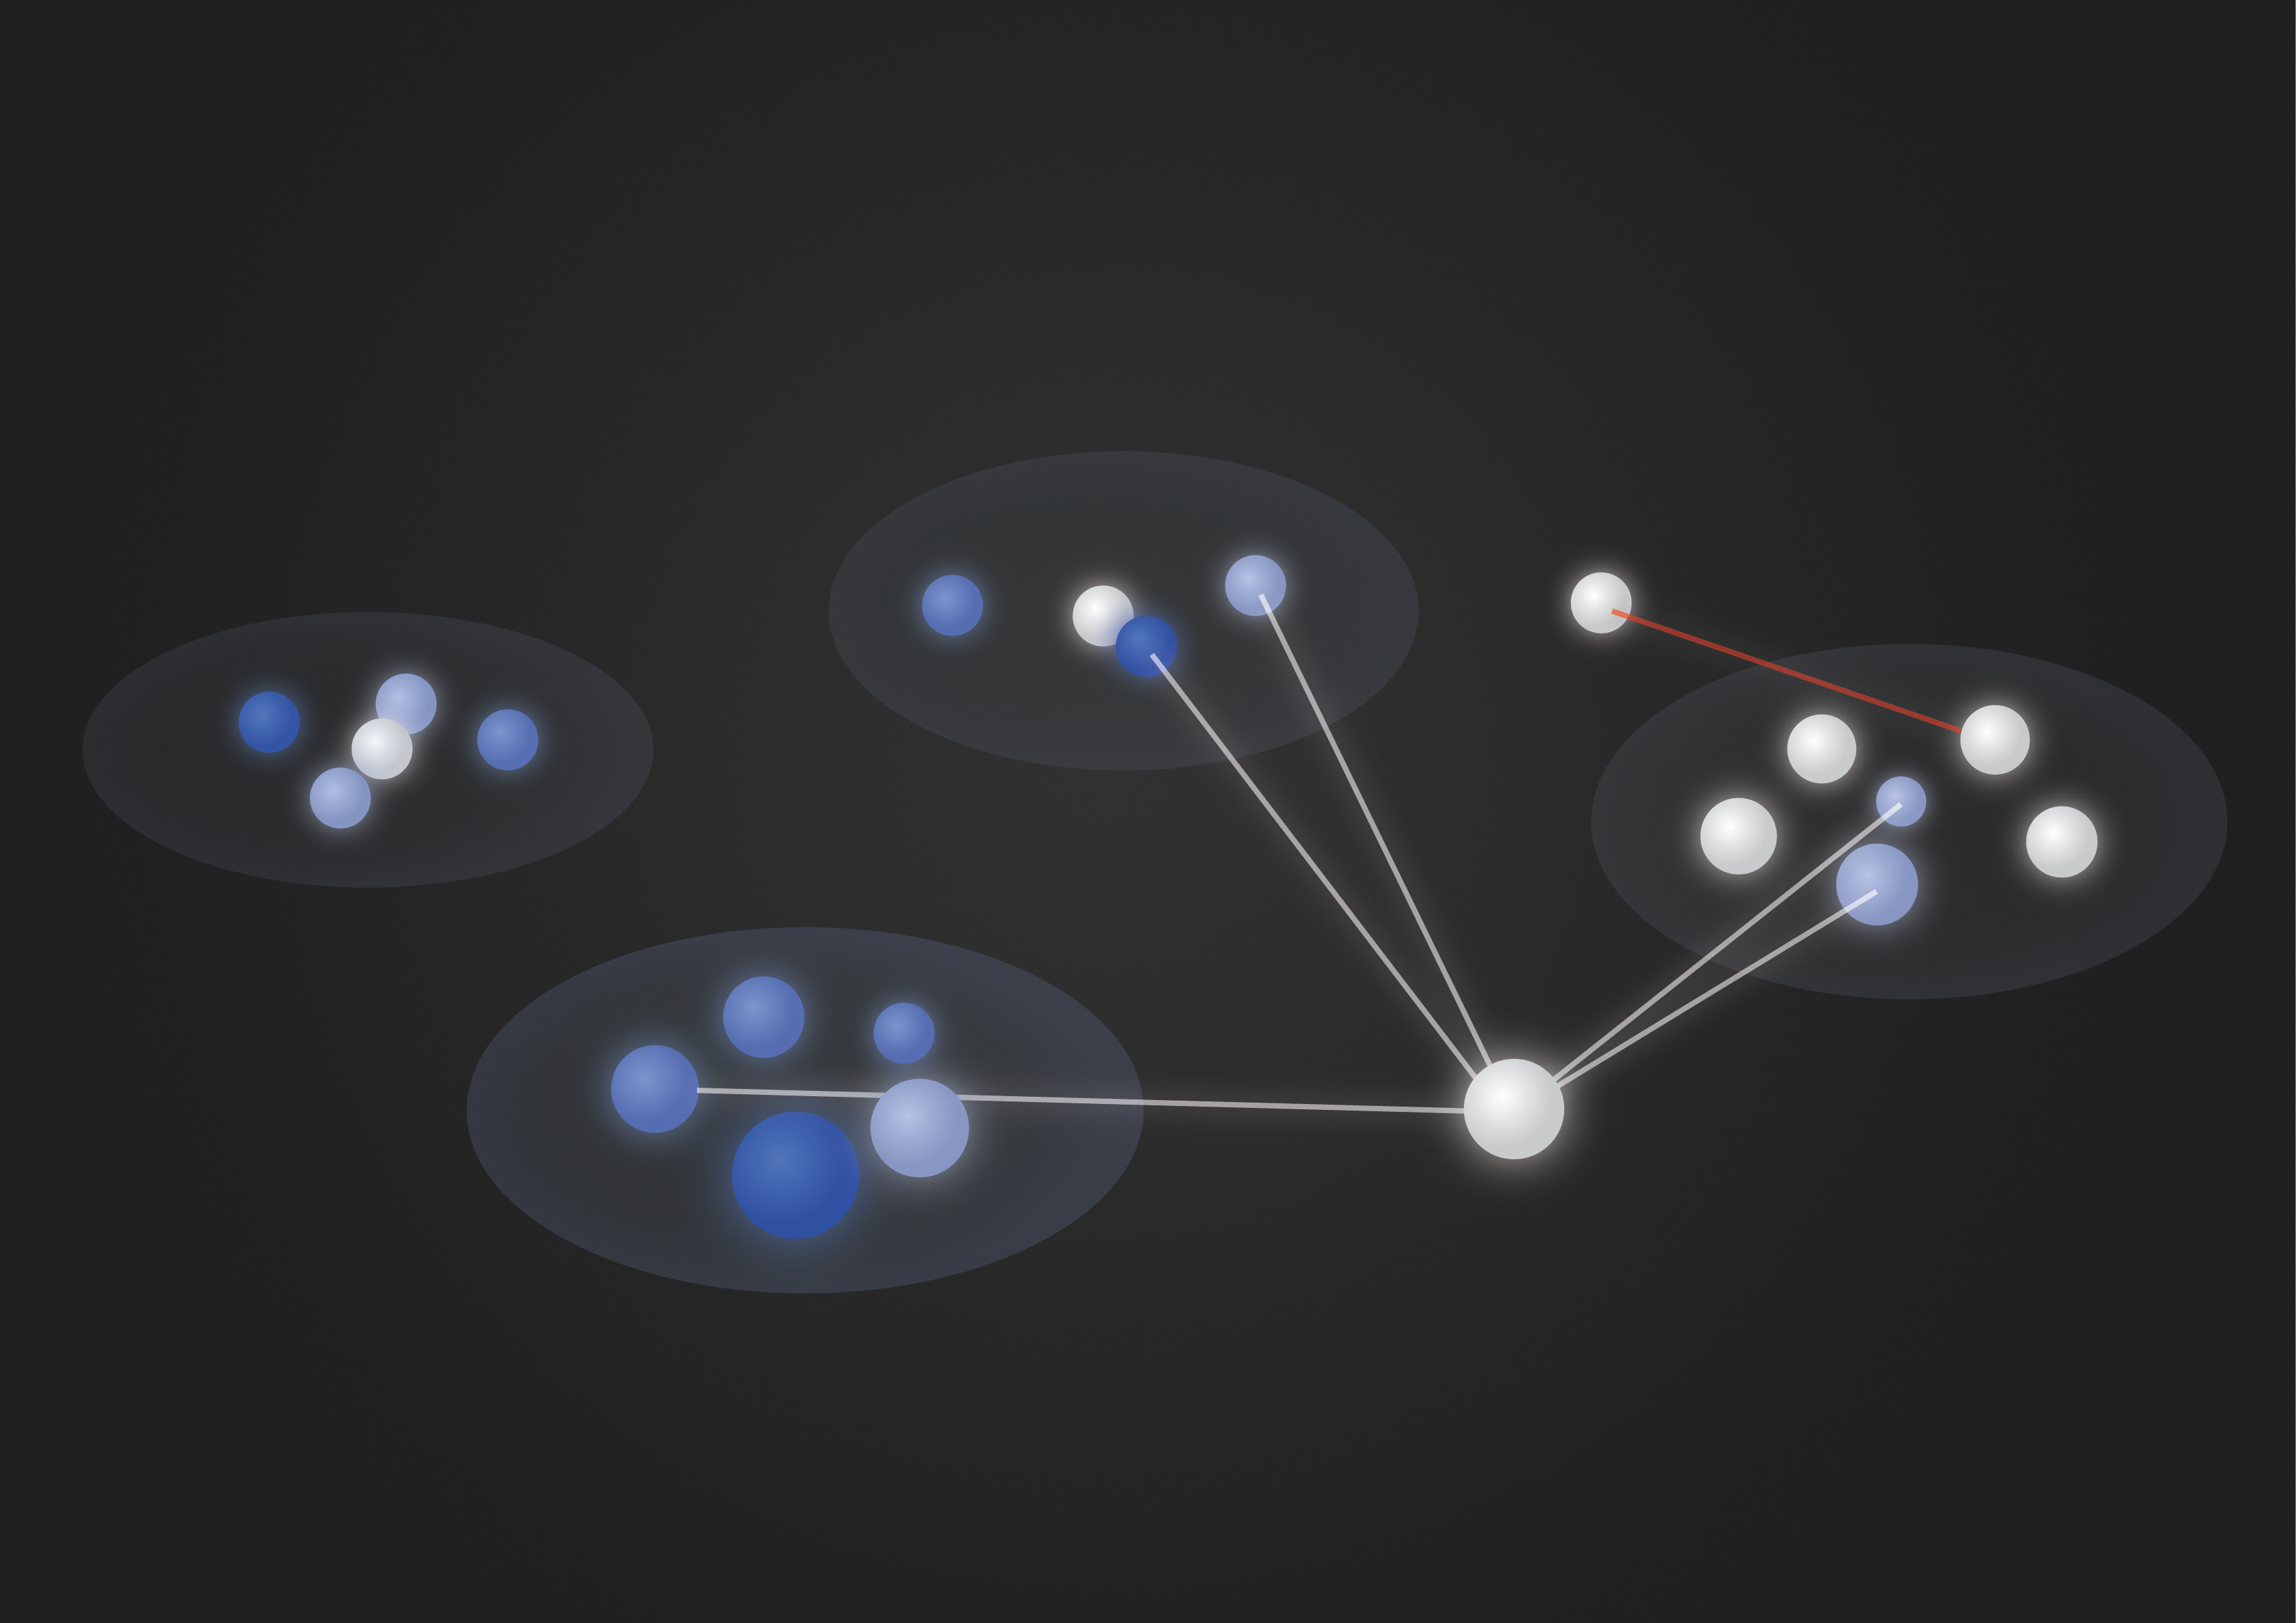
\includegraphics[width=\linewidth]{figures/code-universe}
	\caption{Beispielhafter Entwurf eines CodeUniverse} \label{fig:code-universe}
\end{figure}

\subsubsection*{Nachteile}
Bei der Visualisierung der \textbf{Struktur} einer Software mit dem Modell des CodeUniverse tritt vor allem folgendes Problem auf:

Bei der Abgrenzung der Pakete voneinander mit durchscheinenden, umschließendem Sphären wird von außen betrachtet bei zunehmender Tiefe der Hierarchie zwangsläufig die Blickdichte immer höher. Bei großen Hierarchien kann dies dazu führen, dass die einzelnen Sterne in besonders tiefer Hierarchie nicht mehr gut zu erkennen sind, was sich negativ auf die Übersicht im Bezug auf Größe und Farbe auswirkt. Eine Alternative wäre auf die Sphären zu verzichten. Ob dann die Struktur der Software noch gut zu erkennen ist, bleibt fraglich.

Die Visualisierung der \textbf{Abhängigkeiten} als direkte Verbindung würde bei großen Software-Systemen, ähnlich wie bei der CodeCity (vgl. Nachteile in \ref{subsec:code-city}), schnell unübersichtlich werden. Die aggregierten Abhängigkeiten setzen aber umschließende Sphären, oder ein anderes Konstrukt für $\Psi$ voraus. Würde ein Punkt als $\Psi$ verwendet werden, entstünde ein Bild, ähnlich wie das, das in Abbildung \ref{fig:gource}. Dies ist ein Ausschnitt aus der Visualisierungssoftware namens \textit{Gource} und kommt gut mit zwei Dimensionen aus. 

Ein Vorteil würde nur entstehen, wenn die Verbindungen in die dritte Dimension gezogen würden. Mit etwas Vorstellungskraft lässt sich feststellen, dass so ein Baum entstehen würde. Damit wären wir aber wieder beim CodeForest angelangt und die Metapher eines Universums wäre auch sehr weit her geholt. Abhängigkeiten können also nur sinnvoll als direkte Verbindung realisiert werden.

\begin{figure}[htbp]
	\centering
	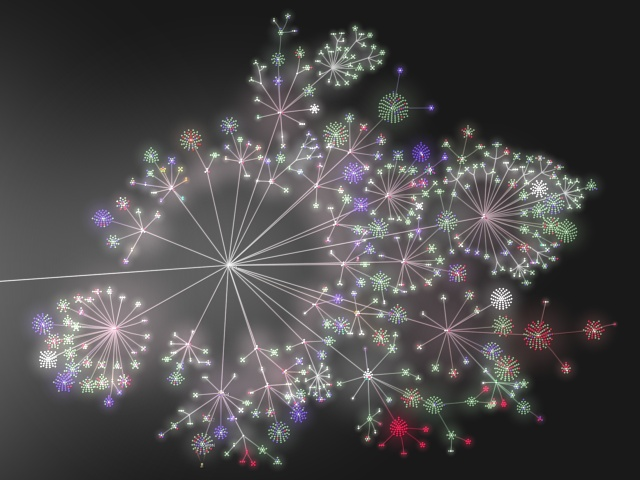
\includegraphics[width=0.5\linewidth]{figures/gource}
	\caption[Visualisierung von Versionskontrolle mit Gource]{Visualisierung von Versionskontrolle mit Gource\protect\footnotemark} \label{fig:gource}
\end{figure}
\footnotetext{Quelle: \url{http://static.oschina.net/uploads/img/201311/15091800_qVuS.jpg}}

\section{Technische Machbarkeit für die Microsoft HoloLens}
\label{sec:technologie}

Es wurde bereits in Abschnitt \ref{subsec:code-city} erörtert, dass sich die CodeCity technologisch nicht eignet auf die HoloLens zu portieren. Im Folgenden soll erprobt werden, ob die bisherige Implementierung von SoftVis3D technisch sinnvoll und mit tragbarem Aufwand auf die HoloLens gebracht und erweitert werden kann.

Die JavaScript Graphik-Bibliothek WebGL wird in \textit{Holographic Windows} von Windows stand 2017 nicht offiziell unterstützt. Es gibt jedoch das open-source Repository \textit{HoloJS} von Microsoft, dass einen experimentellen Support verspricht. Dieses Projekt wandelt mithilfe von C++ jegliche WebGL- in native \textit{DirectX}-Aufrufe\footnote{"`DirectX ist ein Satz von Komponenten in Windows, mit dessen Hilfe Software, und zwar in erster Linie und insbesondere Spiele, Ihre Video- und Audiohardware direkt verwenden kann.  Spiele, die DirectX nutzen, können in Ihre Hardware integrierte Funktionen zur Multimediabeschleunigung effizienter nutzen, wodurch das Multimediaerlebnis insgesamt verbessert wird."' \cite{microsoft2017directx}} um.

Nach anfänglichen Schwierigkeiten und Rücksprache mit einem Microsoft-Entwickler, konnte erfolgreich eine erste Beispiel-App mit three.js auf die HoloLens deployed werden.

Leider erkennet die \textit{Live Preview} oder auch Screenshots der HoloLens die three.js-Objekte nicht und deshalb kann die Beispiel-App in dieser Arbeit nicht veranschaulicht werden.

Was bei der Ausführung der Beispiel-App sofort ins Auge sticht, ist, dass der Curser der HoloLens, ein Punkt im Raum, der der Bewegung des Kopfes folgt oder mit einer verbundenen Zeigergerät bewegt werden kann, doppelt dargestellt wird. Eine sinnvolle Interaktion mit einer three.js-App ist somit nicht ohne Bugfixes möglich.

Nach Aussage von des Microsoft-Entwicklers ist eine aktive Weiterentwicklung des Projekts nicht geplant. Zwar wären Contributions zum HoloJS-Repository möglich, in welchem Umfang dies nötig wäre, um mit three.js-Objekten interagieren zu können, ist jedoch nicht absehbar.

Die Voraussetzung für die Portierung des Frontends von SoftVis3D auf die HoloLens kann deshalb nicht ohne erheblichen und nicht genau kalkulierbaren Aufwand gewährleistet werden.

\todo[inline]{Absatz zu dem Standard-Entwicklungs-Workflow mit Unity und VisualStudio}

\section{Fazit}
\subsection{Vergleich der behandelten Ansätze}
Als Fazit soll eine Empfehlung für die Entwicklung einer Softwarevisualisierung für die HoloLens gegeben werden.

Die CodeCity von Wettel und Lanza stellt erstmals die Stadt-Metapher vor und ist als Konzept sehr durchdacht. Die Verwendung der Implementierung der CodeCity für die HoloLens ist aufgrund der veralteten Technologien jedoch ausgeschlossen. Darüber hinaus hat das Modell auch Schwächen, wie beispielsweise die wenig interaktiv gestaltete und eher unübersichtliche Darstellung der Abhängigkeiten.

SoftVis3D ist als weitere Implementierung der Stadt-Metapher sehr ausgereift und im Gegensatz zu CodeCity mit modernen Web-Technologien gebaut. Die statischen Metriken von Software-Artefakten können hervorragend analysiert werden. Für den Einsatz auf der HoloLens ist SoftVis3D jedoch, wie in \ref{sec:technologie} erläutert, auch nicht geeignet. Die Unterstützung von WebGL ist von Microsoft Stand heute nicht ausreichend gegeben. Das Konzept der Darstellung der Abhängigkeiten in SoftVis3D ist sogar noch unübersichtlicher, als in der CodeCity.

Bei der Betrachtung der zwei vorgestellten Modelle der Stadt-Metapher wäre es natürlich möglich eine neue Implementierung mit den Vorteilen aus beiden Modellen speziell für die HoloLens zu entwickeln und um fehlende Metriken erweitern. Das würde jedoch die wenig attraktive Darstellung der Abhängigkeiten nicht lösen. Zudem wäre sehr viel Aufwand nötig, bis eine neue Softwarevisualisierung überhaupt die Fähigkeiten von SoftVis3D unterstützen würde.

Das CodeUnivers ist ein interessanter und intuitiver Ansatz. Die Struktur ist bei genauerer Betrachtung jedoch schwierig zu realisieren und letztendlich gelangt man bei der Einführung von Abhängigkeiten in das Modell zu einem ähnlichen Konstrukt wie das Modell des CodeForest.

Der CodeForest kann zwar nur eine statische Metrik gleichzeitig anzeigen und lässt deswegen den Zusammenhang zweier Metriken nicht auf einen Blick erkennen, ist aber in allen anderen Bereichen besser bzw. zumindest gleichwertig wie die Alternativen zu bewerten.

\definecolor{good}{hsb}{.3 .4 .9}
\definecolor{poor}{hsb}{0 .4 1}
\newcommand{\cellc}[1]{\cellcolor{good!#1!poor}}
\renewcommand{\tableheader}{
	& \textbf{CodeCity} & \textbf{SoftVis3D} & \textbf{CodeForest} & \textbf{CodeUniverse}\\
}
\begin{tabularx}{\textwidth}{LCCCC}
	\caption{Vergleich der behandelten Ansätze}\label{tab:overview} \\
	\tableheader
	Statische Metriken& \cellc{75}drei gleichzeitig, kaum konfigurierbar & \cellc{100}drei gleichzeitig, sehr flexibel & \cellc{25}nur eine gleichzeitig & \cellc{50}zwei gleichzeitig \\
	Struktur & \cellc{75}übersichtlich & \cellc{100}unterschied\-liche Layouts unterstützt & \cellc{100}durch Baumstruktur sehr gut & \cellc{50}Paket-Zughörigkeit weniger eindeutig \\
	Abhängig\-keiten & \cellc{50}wenig interaktiv, unübersichtlich & \cellc{25}sehr unübersichtlich & \cellc{100}sehr gut darstellbar & \cellc{50}Aggregation schwierig\\
	Dynamik & \cellc{0}nein & \cellc{0}nein & \cellc{100}ja & \cellc{100}ja \\
	Evolution & \cellc{100}sehr gut & \cellc{0}nein & \cellc{100}Wachstum der Bäume & \cellc{50}Ausbreitung des Universums, Entstehung Sterne \\
	Habitability & \cellc{75}gut & \cellc{75}gut & \cellc{100}vertraute Struktur & \cellc{50}weniger markant \\
	Drilldown & \cellc{50}nicht interaktiv & \cellc{75}gut & \cellc{75}gut & \cellc{100}sehr gut\\	
	Technologie & \cellc{0}nicht mehr produktiv einsetzbar & \cellc{50}WebGL   für HoloLens & \cellc{100}neue Technologien einsetzbar & \cellc{100}neue Technologien einsetzbar
\end{tabularx}

Ein Überblick über die in dieser Arbeit aufgestellten Kategorien und die Bewertung der vorgestellten Modelle der dreidimensionalen Softwarevisualisierung darin, ist in Tabelle \ref{tab:overview} zu sehen.

Das Modell des CodeForest ist vielversprechend. Es kann all die Metriken visualisieren, die bei der Umfrage in Abschnitt \ref{subsec:metrics} als wichtig erachtet wurden. Ob Softwareentwickler oder Projektleiter -- alle in der Umfrage vorkommenden Rollen könnten in einem CodeForest wichtige und wertvolle Informationen gewinnen.

\subsection{Ausblick}

In einer weiterführenden Arbeit ist es geplant einen CodeForest für die HoloLens zu entwickeln. Dabei kann auf den Standart-Workflow in der HoloLens-Entwicklung gesetzt werden.

Es ist ein Datenmodell zu entwerfen, dass statische, dynamische und Informationen zur Evolution einer Software unterstützt. Des Weiteren müssen geeignete Algorithmen für das Layout der dreidimensionalen Bäume gefunden werden.

Ein wichtiger Bestandteil einer weiterführenden Arbeit ist die Ausarbeitung des Interaktionskonzepts. Zum Beispiel die Realisierung eines verschiebbaren Waldbodens, wäre eine spannende Aufgabe. Vor allem aber muss das Interaktionsskonzept auch mehrere gleichzeitige Nutzer unterstützen. Durch die SharedView der HoloLens sollte das ein großer Vorteil gegenüber herkömmlichen Softwarevisualisierungen darstellen.

 


\listoffigures

\appendix

\printbibliography

\end{document}
